 \chapter{Matrix Element Analysis Method}
 \label{matrixelement}

This chapter provides the motivation and explanation of a technique known as the matrix element method, which uses probabilities based on leading order matrix elements to extract the single top signal in the dataset. The matrix element method is employed after event selection because the signal to background ratio is $\sim1:20$ thus making an observation of single top impossible. Section~\ref{memotivation} motivates the matrix element method and explains how it is applied to the single  top search. The result of the matrix element method is a set of probabilities for each event to originate from either a signal or background process. The definition and derivation of these probabilities is given in Section~\ref{epd}. Section~\ref{perform} shows the expected separation power between signal and background events using the matrix element method. A comparison of data with the background expectation is shown in Section~\ref{crosscheck} for a data sample where the expected signal fraction is negligible. The result of this comparison shows that the data and background estimation agree after applying the matrix element discriminant. Finally, Section~\ref{matrixelementresults} shows a comparison of data with the expectation for all events.

\section{Motivation and Introduction to the Matrix Element Method}
\label{method-overview}
\label{memotivation}

The measurement of a process with a low rate such as single top quark production requires advanced methods to reduce background rates while keeping signal acceptance high. $\dzero$ has previously published two analyzes using decision trees and neural networks~\cite{Abazov:2005zz,Abazov:2006uq} and released preliminary results using a likelihood discriminant method~\cite{run2-d0-370}. All three of these methods combine differential distributions, that show discrimination between signal and background events, to form a variable which attempts to maximally separated the signal and background. For example, one famous differential distribution that is quite different in signal and background events is the charge of the lepton from the $W$~boson decay multiplied by the $\eta$ of the forward un-tagged jet. This distribution is shown for $t$-channel single top and $Wb\bar{b}$ production in Fig.~\ref{qtimeseta}.

\begin{figure}[!h!tbp]
\begin{center}
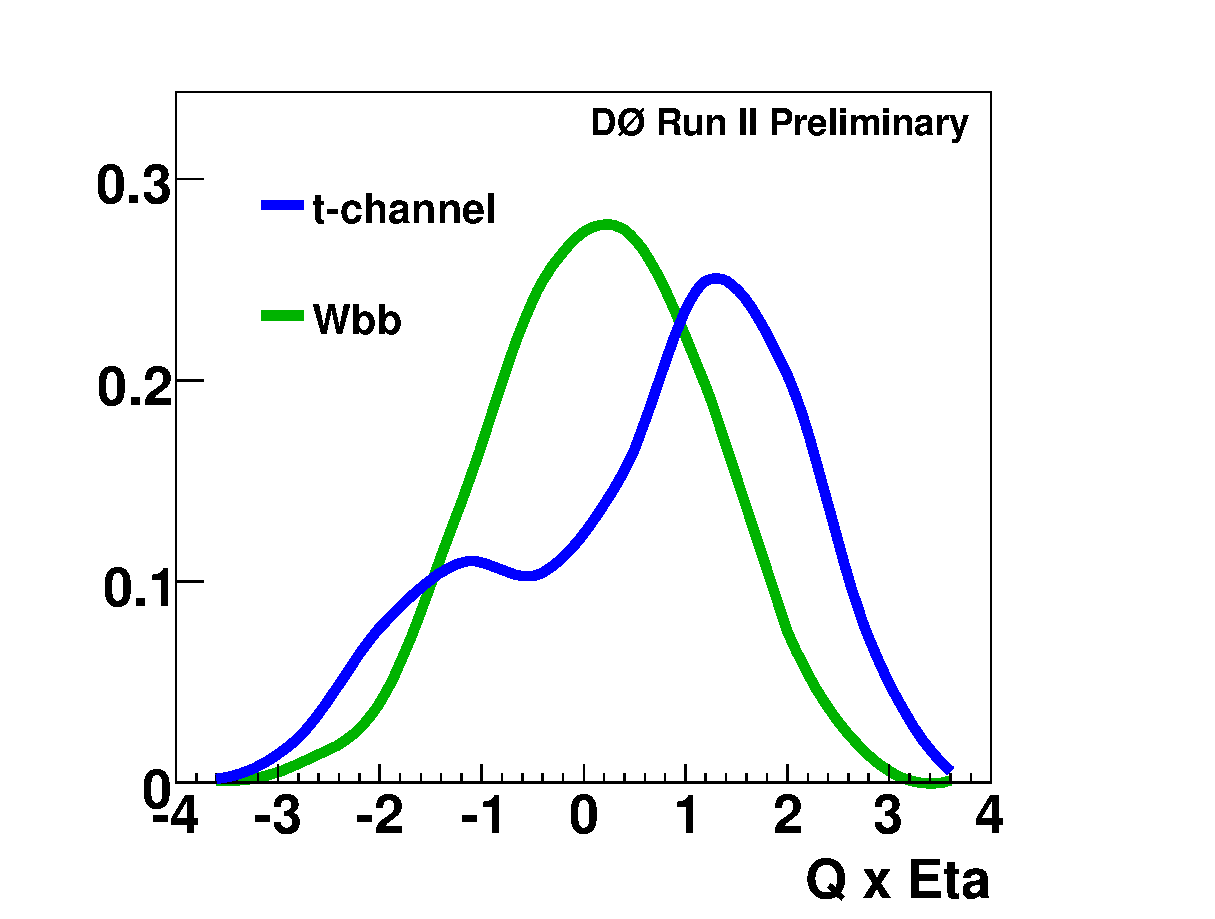
\includegraphics[width=0.75\textwidth]{eps/MatrixElement/intro/qtimeseta.eps}
\vspace{-0.1in}
\caption{Comparison of the lepton charge multiplied by the forward un-tagged jet $\eta$ ($q_{\ell}\times \eta$) for $t$-channel single top (blue) and $Wb\bar{b}$ Monte Carlo events.}
\label{qtimeseta}
\end{center}
\end{figure}

While these methods are very powerful they require~$\emph{a-priori}$~knowledge of the expected correlations in signal and background events. Searching for these correlations is time consuming and if all correlations are not exploited in the analysis it will lead to sub-optimal separation power.

The matrix element method attempts reproduce all correlations present in both signal and background events by weighting events based on the normalized $N$-dimensional differential cross section\footnote{$N$ is the number of independent observables in the event.} at the detector level for both signal and background processes, as shown in Eq.~\ref{define}. 

\begin{equation}
\label{define}
P_{S|B}(\vec{x}) = \frac{1}{\sigma} \frac{d^{N}\sigma_{S|B}}{dx^{N}}
\end{equation}

The number independent observables ($N$) in the event depends on the number of observed particles. For example, an event in the single top dataset will have one lepton, large missing $E_{T}$ and two or three jets\footnote{Events with four jets are not used in this analysis.} resulting in $3 (p_{x},p_{y},p_{z}) \times 3(4)~\rm{particles}=9(12)$ d.o.f for events with two(three) jets. Since the missing E$_{T}$ is indirectly measured from momentum balance with the lepton and jets it is not an independent quantity and therefore not used in the method.

The normalized differential cross sections for signal and background processes are combined using the~$\emph{a-posteriori}$~Bayesian probability density for the signal hypothesis to be true given the measured event $\vec{x}$ as shown in Eq.~\ref{discriminantdef}

\begin{equation}
\label{discriminantdef}
D_{S}(\vec{x}) = P(S|\vec{x}) = \frac{P_S(\vec{x})}{P_S(\vec{x}) + P_B(\vec{x})}
\end{equation}

The remainder of this chapter describes how the differential cross section and normalization are calculated for the signal and background.

\section{Event Probability Density, P$_{S|B}$($\vec{x}$)}
\label{epd}

\subsection{Differential Cross Section Definition}
\label{diffcrosssection}

The differential cross section at the detector level, $\frac{d\sigma}{d\vec{x}}$, is given in
Eq.~\ref{dsigma}; it is defined as the integration over the initial and final state particles' phase space weighted by the differential cross section at the parton level convoluted with a conditional probability to observe event $\vec{x}$ given a particular parton-level state ($\vec{y}$). All quantities in this equation are explained below.

\begin{equation}
\label{dsigma}
\frac{d\sigma}{d\vec{x}} = \sum_{i,j} \int d\vec{y}
\left[ f_{i}(q_{1}, Q^{2})dq_{1}
\times f_{j}(q_{2}, Q^{2})dq_{2}
\times \frac{d\sigma_{hs,ij}}{d\vec{y}}
\times W(\vec{x},\vec{y})
\times \Theta_{\rm{Parton}}(\vec{y}) \right]
\end{equation}


\begin{itemize}
\item $\sum_{i,j}$ is a sum of initial parton flavors in the hard
scatter collision. For example, an $s$-channel collision can occur via
$u\bar{d}$, $c\bar{s}$, $d\bar{u}$, or $s\bar{c}$ annihilation.

\item $f_{i}(q, Q^{2})$ is the parton distribution function for parton
$i$ carrying momentum $q$,
evaluated at the factorization scale $Q^2$. The scale used for $W$+jets processes is  $Q^2=M_{W}^{2} + \sum_{jets}({m_{i}^2 + p_{T,i}^2})$, where $m_{i}$ are the parton masses and $p_{T,i}$ are the transverse momenta of the partons. The scale used for
$s$-channel events is $Q^2=m_t^2$ and scale for $t$-channel events is $Q^{2} = \left( \frac{m_{t}}{2} \right)^{2}$. This analysis uses
CTEQ6~\cite{Pumplin:2005rh} leading-order parton distribution
functions accessed via LHAPDF~\cite{Bourilkov:2006cj}.

\item $\frac{d\sigma_{hs,ij}}{d\vec{y}}$ is the
differential cross section for the hard scatter collision and is solely a function of the initial and final state four-vectors $\vec{y}$. This
quantity is proportional to the square of the leading order matrix
element, as shown in Eq.~\ref{dsigma_hs}:
\begin{equation}
\label{dsigma_hs}
d\sigma_{hs}
= \frac{(2\pi)^4}{4\sqrt{(q_{1}q_{2})^2 - m_{1}^2m_{2}^2}}
|{\cal M}|^{2}
d\Phi_{n}(\vec{y})
\end{equation}
\noindent where the first term is the flux factor, the second term is
the matrix element squared, and the third term is the $n$-body phase
space factor, with $n=4(5)$ for two-jet (three-jet) events, as defined in Eq.~\ref{phasespace}. 

\begin{equation}
\label{phasespace}
d\Phi_{n}(\vec{y}) = \delta^{4}(P - \sum_{i=1}^{n}p_{i}) \prod_{i=1}^{n} \frac{d^{3}p_{i}}{(2\pi)^{3}2E_{i}}
\end{equation}

Matrix elements in this analysis were obtained from the
Madgraph~\cite{Maltoni:2002qb} leading-order matrix-element generator. The signal and background matrix elements depend on the the number of reconstructed jets in the event. Events with two jets are integrated using five matrix elements: two signals ($s$-channel and $t$-channel) and three backgrounds ($Wb\bar{b}$,~$Wcg$, and~$Wgg$). Events with three jets are integrated using three matrix elements: two signals ($s$-channel and $t$-channel and one background ($Wbbg$). The Feynman diagrams for the two and three jet processes are shown in Figs.~\ref{2jets} and~\ref{3jets}, respectively.

\begin{figure}[!h!tbp]
\begin{center}
\includegraphics[width=0.30\textwidth]{eps/MatrixElement/feynman/tb}
\includegraphics[width=0.30\textwidth]{eps/MatrixElement/feynman/tq}\\
\includegraphics[width=0.30\textwidth]{eps/MatrixElement/feynman/wbb}
\includegraphics[width=0.30\textwidth]{eps/MatrixElement/feynman/wcg}
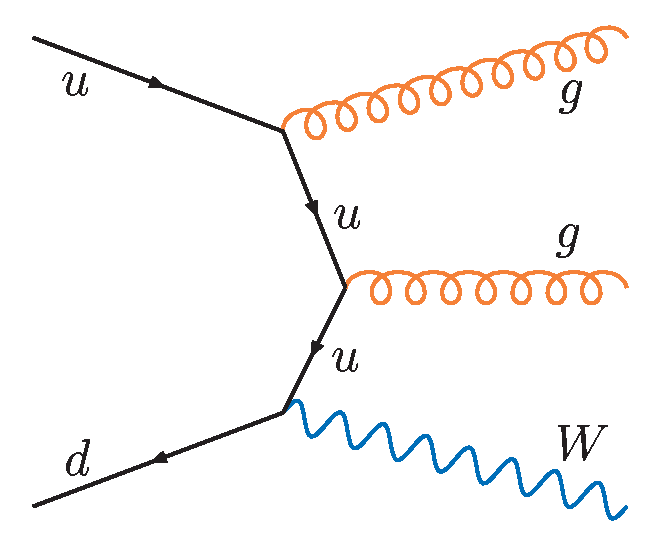
\includegraphics[width=0.30\textwidth]{eps/MatrixElement/feynman/wgg}
\caption{Representative Feynman diagrams corresponding to 
the leading-order matrix elements used for event probability
calculation for events with exactly two jets. Upper row are signals:
$ud{\rightarrow}tb$ and $ub{\rightarrow}td$; lower row are backgrounds: $ud{\rightarrow}Wbb$,
$sg{\rightarrow}Wcg$, and $ud{\rightarrow}Wgg$.}
\end{center}
\label{2jets}
\end{figure}

\begin{figure}[!h!tbp]
\begin{center}
\includegraphics[width=0.30\textwidth]{eps/MatrixElement/feynman/tbg}
\includegraphics[width=0.30\textwidth]{eps/MatrixElement/feynman/tqb}
\includegraphics[width=0.30\textwidth]{eps/MatrixElement/feynman/wbbg}
\caption{Representative Feynman diagrams corresponding to 
the leading-order matrix elements used for event probability
calculation for events with exactly three jets. Left two plots:
signals, $ud{\rightarrow}tbg$, $ug{\rightarrow}tbd$; right plot:
background,$ud{\rightarrow}Wbbg$.}
\end{center}
\label{3jets}
\end{figure}

\item $W(\vec{x},\vec{y})$ is called the transfer function, which 
represents the conditional probability to observe a particular state in the detector ($\vec{x}$) given the original parton-level state ($\vec{y}$). The
transfer functions are determined using Monte Carlo where the
true parton-level four-vectors are known. Transfer functions are determined separately for electrons, muons, and jets, and the full event transfer function is defined as a product of each individual object transfer function as shown in Eq.~\ref{transferfactor}. The description of the transfer function for each object is given below.

\begin{equation}
\label{transferfactor}
W(\vec{x},\vec{y}) = \prod_{i=1}^{n}W_{\rm{Type}}(\vec{x}_{i}, \vec{y}_{i})
\end{equation}

\begin{itemize}
\item Jets - The jet transfer functions are determined for three types of jets: jets originating from a light flavor quark or gluon, jets originating from a $b$ quark that do not contain a muon, and jets originating from a $b$ quark that do contain a muon. A jet is considered to originate from a $b$ quark if there is a $B$ meson with $\Delta R<0.15$ from the jet axis. Any jet that fails this requirement, but is matched to a light flavor quark or gluon with the same matching criteria is considered a light flavor jet. For all jet types the polar angle $\theta$ and azimuthal angle $\phi$ are assumed to be same for the jet and parton. This assumption has been verified in the Monte Carlo. This leaves the jet and parton energies, E$_{j}$ and E$_{p}$, as the sole factors with which the transfer functions depend. To minimize the effect of statistical fluctuations, the transfer functions are parameterized using the functional form shown in Eq.~\ref{jettransferparam}. To account for detector effects the transfer functions were also determined in four $\eta^{\rm{det}}$~regions ($0<|\eta|<0.5$,~$0.5<|\eta|<1.0$,~$1.0<|\eta|<1.5$,~$1.5<|\eta|<3.5$).
\begin{equation}
\label{jettransferparam}
W_{\rm{Jet}}(E_{p},E_{j}) = N \times \left[ \mathrm{exp}\left\{\frac{-(\Delta E-\alpha_{1})^{2}}{2p^{2}_{2}}\right\} + \alpha_{3}\mathrm{exp} \left\{\frac{-(\Delta E-\alpha_{4})^{2}}{2p^{2}_{5}} \right\}		\right] \\
\end{equation}

\begin{eqnarray}
\nonumber
N = \frac{1}{\sqrt{2\pi}(\alpha_{2} + \alpha_{3}\alpha_{5})}
\end{eqnarray}

\noindent Where $\Delta E=E_{j}-E_{p}$ and $\alpha_{i} = a_{i}+b_{i} \times E_{p}$. For each of the three jet types and each of the four detector regions the transfer function parameters are determined by minimizing the logarithm of the likelihood function, shown in Eq.~\ref{tfloglikelihood}.

\begin{equation}
\label{tfloglikelihood}
L(\vec{\alpha}) = \prod_{i=1}^{N_{\rm{Events}}}W(\vec{\alpha}, E_{p}^{i}, E_{j}^{i})
\end{equation}

The values of $\vec{\alpha}$ for light jets, $B$-jets, and $B$-jets~w/ $\mu$ can be found in Tables~\ref{lightjettfparams},~\ref{bjettfparams}, and~\ref{bmujettfparams}. A plot of $\Delta E$ for all jets used to determine the transfer function parameters is shown in Fig.~\ref{FlavorTF}.

\begin{figure}[!h!tbp]
\begin{center}
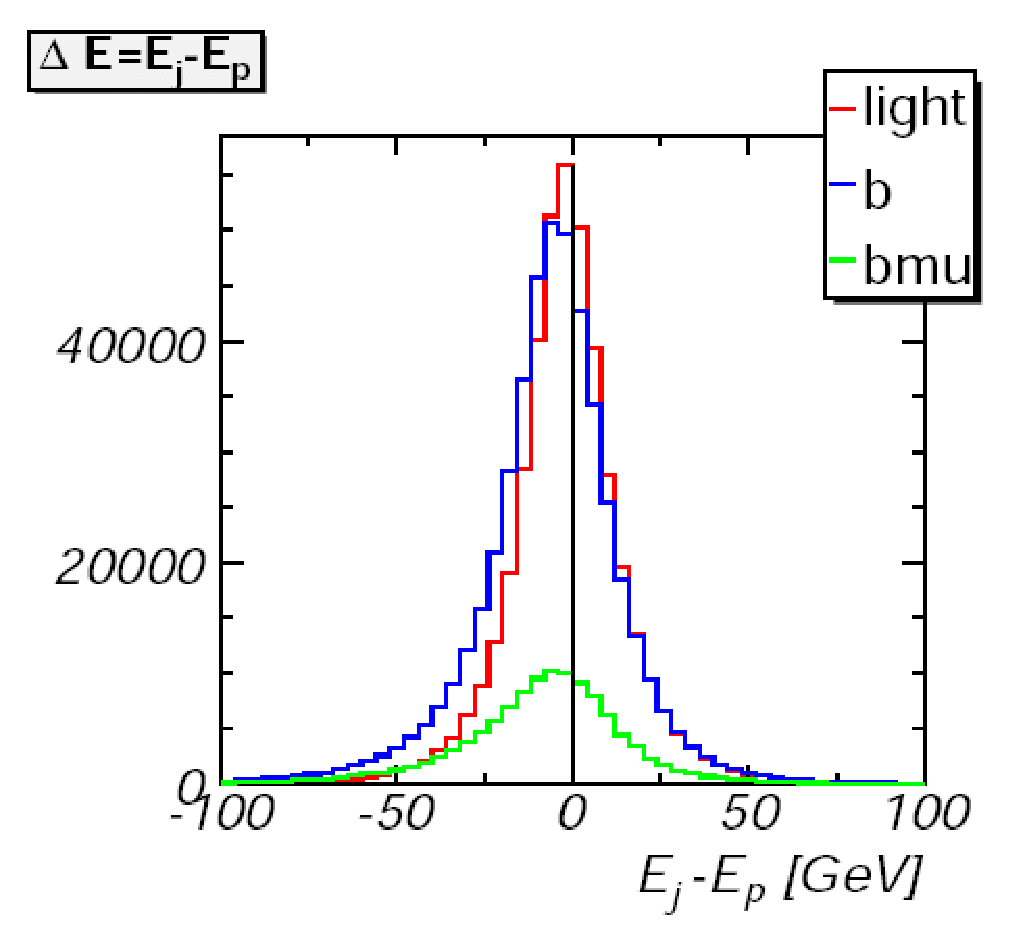
\includegraphics[width=0.75\textwidth]{eps/MatrixElement/transfer/tfs}
\vspace{-0.1in}
\caption{Energy difference between a reconstructed jet and its matched parton
for three types of jets for all eta regions and all jet energies.}
\label{FlavorTF}
\end{center}
\end{figure}


\begin{table}[!h!tbp]
\begin{center}
\caption{Light jet transfer function parameters.}
\label{lightjettfparams}
\begin{tabular}{c|cc|cc|cc|cc|cc}
%\multicolumn{11}{c}
%{\underline{Light Jet Transfer Function Parameters}} \\
&	\multicolumn{2}{c|}{$\alpha_{1}$}		& \multicolumn{2}{c|}{$\alpha_{2}$} 
&	\multicolumn{2}{c|}{$\alpha_{3}$}		& \multicolumn{2}{c|}{$\alpha_{4}$} 
&	\multicolumn{2}{c}{$\alpha_{5}$}		\\
				& 	$a$	&	$b$	&	$a$	&	$b$	& 	$a$	&	$b$	& 	$a$	&	$b$	& 	$a$	&	$b$	\\	
\hline
$0.0<|\eta|<0.5$	& -4.17	& 0.04	& 4.12	& 0.11	& 0.0		& 0.0013	& 24.8	& -0.19	& 15.6	& 0.23	\\
$0.5<|\eta|<1.0$	& -2.90	& 0.03	& 5.26	& 0.12	& 0.0		& 0.0010	& 57.3	& -0.47	& -16.1	& 0.69	\\
$1.0<|\eta|<1.5$	& -0.61	& 0.02	& 8.16	& 0.13	& 0.0		& 0.0010	& 70.7	& -0.37	& -11.5	& 0.54	\\
$1.5<|\eta|<3.5$	& 3.12	& -0.06	& 12.4	& 0.11	& 0.0		& 0.0011	& 234	& -1.53	& -22.3	& 0.49	\\
\end{tabular}
\vspace{-0.1 in}
\end{center}
\end{table} 


\begin{table}[!h!tbp]
\begin{center}
\caption{$B$ jet transfer function parameters.}
\label{bjettfparams}
\begin{tabular}{c|cc|cc|cc|cc|cc}
%\multicolumn{11}{c}
%{\underline{$B$ Jet Transfer Function Parameters}} \\
&	\multicolumn{2}{c|}{$\alpha_{1}$}		& \multicolumn{2}{c|}{$\alpha_{2}$} 
&	\multicolumn{2}{c|}{$\alpha_{3}$}		& \multicolumn{2}{c|}{$\alpha_{4}$} 
&	\multicolumn{2}{c}{$\alpha_{5}$}		\\
				& 	$a$	&	$b$	&	$a$	&	$b$	& 	$a$	&	$b$	& 	$a$	&	$b$	& 	$a$	&	$b$	\\	
\hline
$0.0<|\eta|<0.5$	& -5.61	& 0.01	& 3.27	& 0.14	& 0.0		& 0.0018	& 49.9	& -0.77	& 32.7	& -0.03	\\
$0.5<|\eta|<1.0$	& -4.07	& 0.01	& 3.31	& 0.15	& 0.0		& 0.0018	& 52.1	& -0.76	& 41.1	& -0.09	\\
$1.0<|\eta|<1.5$	& -1.92	& -0.06	& 6.46	& 0.15	& 0.0		& 0.0011	& 98.8	& -0.74	& -17.0	& 0.64	\\
$1.5<|\eta|<3.5$	& -0.87	& -0.07	& 5.84	& 0.17	& 0.0		& 0.0011	& -5.84	& -0.98	& -5.83	& 0.39	\\
\end{tabular}
\vspace{-0.1 in}
\end{center}
\end{table} 


\begin{table}[!h!tbp]
\begin{center}
\caption{$B$~w/$\mu$ jet transfer function parameters.}
\label{bmujettfparams}
\begin{tabular}{c|cc|cc|cc|cc|cc}
%\multicolumn{11}{c}
%{\underline{$B$~w/$\mu$ Jet Transfer Function Parameters}} \\
&	\multicolumn{2}{c|}{$\alpha_{1}$}		& \multicolumn{2}{c|}{$\alpha_{2}$} 
&	\multicolumn{2}{c|}{$\alpha_{3}$}		& \multicolumn{2}{c|}{$\alpha_{4}$} 
&	\multicolumn{2}{c}{$\alpha_{5}$}		\\
				& 	$a$	&	$b$	&	$a$	&	$b$	& 	$a$	&	$b$	& 	$a$	&	$b$	& 	$a$	&	$b$	\\	
\hline
$0.0<|\eta|<0.5$	& -1.38	& -0.06	& 3.65	& 0.16	& 0.0		& 0.0017	& 55.7	& -0.46	& 91.5	& -0.16	\\
$0.5<|\eta|<1.0$	& -0.37	& -0.07	& 4.30	& 0.16	& 0.0		& 0.0014	& 110	& -0.93	& -4.56	& 0.66	\\
$1.0<|\eta|<1.5$	& 2.61	& -0.11	& 5.42	& 0.17	& 0.0		& 0.0015	& 119	& -0.91	& -9.31	& 0.39	\\
$1.5<|\eta|<3.5$	& 12.9	& -0.20	& 4.17	& 0.19	& 0.0		& 0.0024	& 215	& -1.39	& 42.3	& 0.17	\\
\end{tabular}
\vspace{-0.1 in}
\end{center}
\end{table} 





\item Electrons - The transfer function for electrons is assumed to be
solely a function of the reconstructed energy of the electron,
$E_{e}$, the parton-level energy of the electron, $E_{p}$, and
$\theta$, the production angle with respect to the beam axis. The transfer function is parameterized by a Gaussian in the relative energy difference with a width that depends on the reconstructed energy and the production angle. This functional form is shown in Eq.~\ref{electrontf}.

\begin{equation}
\label{electrontf}
W(E_{e}, E_{p}, \theta) = \frac{1}{2\pi\sigma}\mathrm{exp}\left\{-\frac{(E_{e} - \alpha_{1}\times E_{p} - \alpha_{2})^{2}}{2\sigma^{2}}\right\}\\
\end{equation}

\noindent Where the Gaussian width $\sigma$ is defined as the product of a parton energy error term, a sampling error term, and a constant error term as shown in Eq.~\ref{electronerrortf}. The values of $\vec{\alpha}$ in the electron transfer function are shown in Table~\ref{electrontfparams}.

\begin{eqnarray}
\label{electronerrortf}
\nonumber
\sigma & = &
\alpha_{3} E_{\rm{cen}}~\times~\textrm{Sampling}(E_{\rm{cen}},\theta) E_{\rm{cen}}~\times~\alpha_{4} \\
\nonumber
E_{\rm{cen}} & = &
\alpha_{1} E_{p} + \alpha_{2} \\
\nonumber
\textrm{Sampling}(E_{e}, \theta) & = &
\left[\frac{\alpha_{5}}{\sqrt{E_{e}}} + \frac{\alpha_{6}}{E_{e}}\right]
\textrm{exp}\left\{\frac{f(E_{e})}
{\textrm{sin}\theta}-f(E_{e})\right\} \\
f(E_{e})& = & \alpha_{7} - \frac{\alpha_{8}}{E_{e}} - \frac{\alpha_{9}}{E_{e}^2}.
\end{eqnarray}

\begin{table}[!h!tbp]
\begin{center}
\caption{Electron transfer function parameters.}
\label{electrontfparams}
\begin{tabular}{cc|cc|cc|ccc}
%\multicolumn{9}{c}
%{\underline{Electron Transfer Function Parameters}} \\
	\multicolumn{2}{c|}{$E_{\rm{cen}}$}		& \multicolumn{2}{c|}{$\sigma$} 
&	\multicolumn{2}{c|}{Sampling} 			& \multicolumn{3}{c}{$f(E)$} \\
 	$\alpha_{1}$	&	$\alpha_{2}$		& $\alpha_{3}$	&	$\alpha_{4}$		
& 	$\alpha_{5}$	&	$\alpha_{6}$		& $\alpha_{7}$	&	$\alpha_{8}$	&	$\alpha_{9}$	\\
\hline
	0.0002	&	0.324	&	0.028	&	0.4	&	0.164	&	0.122	&	1.35	&	2.09	&	6.99	\\
\end{tabular}
\vspace{-0.1 in}
\end{center}
\end{table} 



\item Muons - The muon transfer functions are determined for muons with and without SMT hits and are parameterized using the Gaussian functional form shown in Eq.~\ref{muontf}.

\begin{equation}
\label{muontf}
W\left(\left( \frac{q}{p_t}\right)_{\mu}, \left( \frac{q}{p_t}\right)_{p}, \eta \right) = 
\frac{1}{2\pi\sigma}\mathrm{exp}
\left\{-\frac{\left[\Delta
\left( \frac{q}{p_t} \right)\right]^2}
{2\sigma^2}\right\}
\end{equation}

\noindent Where the Gaussian width $\sigma$ is defined separately for two $\eta$ regions as shown in Eq.~\ref{muonerrortf}. The $\eta$~region dependence is a result of the limited $\eta$ coverage of the central fiber tracker in the forward region.

\begin{equation}
\label{muonerrortf}
\sigma  =  \left\{ 
\begin{array} {c@{\quad:\quad}l} \alpha_{1} &
|\eta| \le 1.4 \\
\sqrt{\alpha^{2}_{1} + [\alpha_{2}(|\eta| - 1.4)]^2} &
|\eta| > 1.4 
\end{array} \right\}
\end{equation}

The parameters $\alpha_{1}$ and $\alpha_{2}$ in the transfer function parameterization contain a constant term and a term proportional to $\frac{1}{p_{T}}$. The four parameters are extracted using a maximum likelihood method similar to the method used to determine the jet transfer function. The muon transfer function parameters are shown in Table~\ref{muontfparams}.

\begin{table}[!h!tbp]
\begin{center}
\caption{Muon transfer function parameters (Eq.~\ref{muontf}) for muons with and without SMT hits.}
\label{muontfparams}
\begin{tabular}{c|cc|cc}
%\multicolumn{5}{c}
%{\underline{Muon Transfer Function Parameters}} \\
       & \multicolumn{2}{|c|}{$\alpha_{1}$} & \multicolumn{2}{|c}{$\alpha_{2}$} \\
Muon Type		& Constant			& $\propto \frac{1}{p_{T}}$	&	Constant			&	$\propto \frac{1}{p_{T}}$		\\
\hline
$=0$ SMT Hits		& 2.96$\times10^{-3}$	& 2.91$\times10^{-2}$		& 1.95$\times10^{-2}$	& -3.04$\times10^{-2}$		\\
$\geq1$ SMT Hit	& 2.07$\times10^{-3}$	& 2.22$\times10^{-2}$		& 5.56$\times10^{-3}$	& 1.19$\times10^{-1}$		\\
\end{tabular}
\vspace{-0.1 in}
\end{center}
\end{table} 

\end{itemize}

\item $\Theta_{\rm{Parton}}(\vec{y})$ represents the parton level
cuts applied to avoid singularities in the matrix element
evaluation. All differential cross sections were calculated with the
following parton level cuts:

\begin{itemize}
\item Parton isolation: $\Delta$R($q_{i}$,$q_{j})>0.5$
\item Minimum parton $P_T$: $P_{T}(q_i)>6$ GeV
\item Maximum parton pseudorapidity: $|\eta(q_i)|<3.5$
\item No cuts are applied to the lepton or neutrino
\end{itemize}

\item $\int d\vec{y}dq_{1}dq_{2}$ is an integration over the phase space defined by the final state particles ($d\vec{y}$) and the two initial parton's longitudinal momentum ($dq_{1},~dq_{2}$). The phase space for a lepton, neutrino, and two parton final state event is defined by 14 degrees of freedom (one momentum (p) and two angles ($\Omega$) for each final state particle plus the two initial parton momenta), as shown in Eq.~\ref{dy}.
\begin{equation}
\label{dy}
d\vec{y}_{\ell\nu q_{1}q_{2}} = dq_{1}dq_{2}d|p|_{\ell}
d\Omega_{\ell}d|p|_{\nu}
d\Omega_{\nu}d|p|_{q1}
d\Omega_{q1}d|p|_{q2}
d\Omega_{q2}
\end{equation}

Events with three partons in the final state have 17 degrees of freedom and has a phase space defined in Eq.~\ref{dy3jet}.
\begin{equation}
\label{dy3jet}
d\vec{y}_{\ell\nu q_{1}q_{2}q_{3}} = dq_{1}dq_{2}d|p|_{\ell}
d\Omega_{\ell}d|p|_{\nu}
d\Omega_{\nu}d|p|_{q1}
d\Omega_{q1}d|p|_{q2}
d\Omega_{q2}d|p|_{q3}
d\Omega_{q3}
\end{equation}

When performing the integration four (six) degrees of freedom are removed for two
(three) parton events by assuming equal azimuthal and polar angles ($\phi$,~$\theta$) for partons and
jets as required by the transfer functions. Two more
degrees of freedom are removed by assuming well measured lepton
angles. Four more degrees of freedom are removed from the integration
by energy-momentum conservation, leaving four(five) integration
variables for events with two(three) jets. The final integration phase space is then transformed to
suit the matrix element being integrated. $W$+jets matrix element
integrations use the phase space defined in Eqs.~\ref{wjets_int} and
single top matrix element integrations use the phase space in
Eq.~\ref{st_int}.

\begin{eqnarray}
\label{wjets_int}
\nonumber
d\vec{y}_{\rm{W+jets - 2jets}} &=& du_{W}d|p_{q1}|d|p_{q2}|dp^{system}_{z}	\\
d\vec{y}_{\rm{W+jets - 3jets}} &=& du_{W}d|p_{q1}|d|p_{q2}|d|p_{q3}|dp^{system}_{z}
\end{eqnarray}

\begin{eqnarray}
\label{st_int}
\nonumber
d\vec{y}_{\rm{single top - 2jets}} &=& du_{t}du_{W}d|p_{q2}|dp^{system}_{z}	\\
d\vec{y}_{\rm{single top - 3jets}} &=& du_{t}du_{W}d|p_{q2}|d|p_{q3}|dp^{system}_{z}
\end{eqnarray}


In Eqs.~\ref{wjets_int} and~\ref{st_int}, $du_{W}$ and $du_{t}$ are used to uniformly sample a Breit-Wigner distribution centered around the $W$ mass and top quark mass, respectively. Because the differential cross section for a $W$+jets process is sharply peaked when the mass of the lepton and neutrino system is near the $W$ mass, integrating solely in this region reduces the integration time considerably. The same reasoning applies to the top quark mass and the mass of the lepton, neutrino, and $b$-quark. The initial parton momentum fractions are transformed into the total system energy and longitudinal momentum. With this choice of integration variables the total energy integral is removed along with the neutrino momentum from energy and momentum conservation. The total longitudinal momentum remains as an integration variable.

When changing integration variables a Jacobian is required to modify the differential cross section. The Jacobians for the $W$+jets and single top change of variable are shown in Eqs.~\ref{wjets_jac2} and~\ref{st_jac2}.\footnote{In all Jacobian equations the subscript 3 refers to the lepton, 4 refers to the neutrino, and 5,6, and 7, refer to the final state partons. The global factor of $\frac{2}{s}$ is a result of the Jacobian for the $q_{1}q_{2} \rightarrow E^{\rm{tot}}P^{tot}_{z}$ change of variables. $s_{\rm{max}}$ is the maximum available mass-squared for the collision and $s_{\rm{min}}$ is the minimum mass-squared required to create the final state particles.}


\begin{eqnarray}
\label{wjets_jac2}
|J(p_{3}, \rightarrow u_{W})| =
\frac{2}{s} \times \Delta S_{W} \times \left| \frac{\left[
(m_{W}\Gamma_{W})^{2} + (m^{2}_{34} - m_{W}^{2})^{2} \right]}{2(p_{3} + p_{4})(1 -
\hat{p_{3}} \cdot \hat{p_{4}})} \right|
\end{eqnarray}

\begin{eqnarray}
\label{st_jac2}
\nonumber
|J(p_{3}, p_{5} \rightarrow u_{W}, u_{t})| &=& 
\frac{2}{s} \times \Delta S_{W} \times \Delta S_{t} \times \\
& & \left| \begin{array}{cc}
\frac{\left[
(m_{t}\Gamma_{t})^{2} + (m^{2}_{345} - m_{t}^{2})^{2} \right]}{2(p_{3} + p_{4} + p_{5})(1 - \hat{p_{3}} \cdot \hat{p_{4}})}	& \frac{\left[
(m_{W}\Gamma_{W})^{2} + (m^{2}_{34} - m_{W}^{2})^{2} \right]}{2(p_{3} + p_{4})(1 -
\hat{p_{3}} \cdot \hat{p_{4}})} \\
\frac{\left[
(m_{t}\Gamma_{t})^{2} + (m^{2}_{345} - m_{t}^{2})^{2} \right]}{2(p_{3} + p_{4} + p_{5})(1 - \hat{p_{4}} \cdot \hat{p_{5}})}	& \frac{\left[
(m_{W}\Gamma_{W})^{2} + (m^{2}_{34} - m_{0}^{2})^{2} \right]}{2p_{3}(\hat{p_{3}} \cdot \hat{p_{5}} - \hat{p_{4}} \cdot \hat{p_{5}})}
\end{array}
\right|
\end{eqnarray}

where $\Delta S_{W}$ and $\Delta S_{t}$ are defined in Eqs.~\ref{deltaSW} and~\ref{deltaStop}.

\begin{eqnarray}
\label{deltaSW}
\Delta S_{W} &=& \left( \frac{1}{m_{W}\Gamma_{W}} \right) \left(  \tan \left[ \frac{s_{\rm{max}} - m_{W}^{2}}{m_{W}\Gamma_{W}} \right] - \tan \left[ \frac{s_{\rm{min}} - m_{W}^{2}}{m_{W}\Gamma_{W}} \right] \right)	\\
\label{deltaStop}
\Delta S_{t} &=& \left( \frac{1}{m_{t}\Gamma_{t}} \right) \left(  \tan \left[ \frac{s_{\rm{max}} - m_{t}^{2}}{m_{t}\Gamma_{t}} \right] - \tan \left[ \frac{s_{\rm{min}} - m_{t}^{2}}{m_{t}\Gamma_{t}} \right] \right)
\end{eqnarray}

\end{itemize}

The multidimensional integrals in this analysis were performed using the GNU Scientific Library version of the VEGAS~\cite{Lepage:1980dq} Monte Carlo integration algorithm. 


\subsection{Probability Normalization Constants}
\label{normalization}

The differential cross section defined in Eq.~\ref{dsigma}
requires a normalization constant to retain a probability density
interpretation. The normalization constant $\sigma$ is defined as the
detector level phase space integration ($\int d\vec{x}$) of the
differential cross section, as shown in Eq.~\ref{cross}.

\begin{equation}
\label{cross}
\sigma = \sum_{i,j} \int d\vec{x}d\vec{y}
\left[ \frac{d\sigma_{i,j}}{d\vec{y}}
\times W(\vec{x},\vec{y})
\times \Theta_{\rm{cuts}}(\vec{x})
\right]
\end{equation}

The term $\Theta_{\rm{cuts}}(\vec{x})$ is included in the calculation to account for the acceptance after selection cuts. This factor is set to one if the event passes the selection cuts and zero if it fails. All normalization constants were calculated with the following selection cuts:

\begin{itemize}
\item Lepton $P_{T}$ $>$ 15 GeV
\item Electron (muon) $|\eta|$ $<$ 1.1(2.0)
\item Missing $E_{T}$ $>$ 15 GeV
\item Leading jet $P_{T}$ $>$ 25 GeV
\item Leading jet $|\eta|$ $<$ 2.5
\item Second jet $P_{T}$ $>$ 20 GeV
\item Second jet $|\eta|$ $<$ 3.5
\item Third jet $P_{T}$ $>$ 15 GeV (if three-jet event)
\item Third jet $|\eta|$ $<$ 3.5 (if three-jet event)
\end{itemize}

The selection cuts shown above are slighty different from the
canonical single top cuts. These cuts are included in the
normalization calculation to approximate the relative acceptance
difference between signal and background events. The cross sections
computed for each signal and background process for two- and three-jet
events are summarized in Table~\ref{cross-sections}. In all instances,
the statistical uncertainty from the Monte Carlo integration is below
$1\%$.

\begin{table}[!h!tbp]
\begin{center}
\caption{Cross section times branching fraction for each
analysis channel. All cross sections are given in units of femtobarns (fb).}
\label{cross-sections}
\begin{tabular}{c|cccc|cccc}
%\multicolumn{9}{c}
%{\underline{Cross Section $\times$ Branching Fraction [fb]}}
%\vspace{0.05in} \\
            & \multicolumn{4}{c|}{2-jet events}
            & \multicolumn{4}{c}{3-jet events} \\
            & \multicolumn{2}{c}{1 tag}
            & \multicolumn{2}{c|}{2 tags}
            & \multicolumn{2}{c}{1 tag}
            & \multicolumn{2}{c}{2 tags}\\
            & Electron &   Muon   & Electron &   Muon
            & Electron &   Muon   & Electron &   Muon   \\
\hline
Signals     &    &     &     &    &    &     &    &     \\
~~$tb(g)$   &   8.07   &   10.4   &   6.90   &   8.90   
            &   6.02   &   7.64   &   5.22   &   6.66   \\
~~$tq(b)$   &  19.6    &   26.8   &   0.27   &   0.38   
            &   6.34   &    8.56  &   5.40   &   7.40   \\
Backgrounds &    &     &     &    &    &     &    &     \\
~~$Wbb(g)$  &  29.5    &   41.9   &  24.6    &  34.7    
            &   16.5   &   23.1   &   14.3   &   19.9   \\
~~$Wcg$     &  36.4    &   54.0   &   0.33   &   0.61   & & & & \\
~~$Wgg$     &  52.3    &   74.5   &   0.33   &   0.47   & & & &  
\end{tabular}
\vspace{-0.1 in}
\end{center}
\end{table}


\subsection{Treatment of Combinatorial Background}
The event probability density shown in Eq.~\ref{dsigma} assumes a known
assignment between a jet and parton from the matrix element. In
practice this assignment is not known so there must be a sum over
all possible assignments. The general treatment of the combinatorial backgrounds for events with two jets is shown in Eq.~\ref{pxcomb} and Eq.~\ref{pxcomb3} for three jet events.

\begin{eqnarray}
\label{pxcomb}
d\sigma(\ell, j_1, j_2)
&=& \alpha_{j_1 {\rightarrow} p_1} \alpha_{j_2 {\rightarrow} p_2}
    d\sigma(\ell, j_1 {\rightarrow} p_1, j_2 {\rightarrow} p_2) + \nonumber \\
&+& \alpha_{j_2 {\rightarrow} p_1} \alpha_{j_1 {\rightarrow} p_2}
    d\sigma(\ell, j_2 {\rightarrow} p_1, j_1 {\rightarrow} p_2) 
\end{eqnarray}

\begin{eqnarray}
\label{pxcomb3}
    \nonumber
d\sigma(\ell, j_1, j_2, j_3)
&=& \alpha_{j_1 {\rightarrow} p_1} \alpha_{j_2 {\rightarrow} p_2} \alpha_{j_3 {\rightarrow} p_3}
    d\sigma(\ell, j_1 {\rightarrow} p_1, j_2 {\rightarrow} p_2, j_3 {\rightarrow} p_3) \\
    \nonumber
&+& \alpha_{j_1 {\rightarrow} p_1} \alpha_{j_3 {\rightarrow} p_2} \alpha_{j_2 {\rightarrow} p_3}
    d\sigma(\ell, j_1 {\rightarrow} p_1, j_3 {\rightarrow} p_2, j_2 {\rightarrow} p_3) \\
    \nonumber
&+& \alpha_{j_2 {\rightarrow} p_1} \alpha_{j_1 {\rightarrow} p_2} \alpha_{j_3 {\rightarrow} p_3}
    d\sigma(\ell, j_2 {\rightarrow} p_1, j_1 {\rightarrow} p_2, j_3 {\rightarrow} p_3) \\
    \nonumber
&+& \alpha_{j_2 {\rightarrow} p_1} \alpha_{j_3 {\rightarrow} p_2} \alpha_{j_1 {\rightarrow} p_3}
    d\sigma(\ell, j_2 {\rightarrow} p_1, j_3 {\rightarrow} p_2, j_1 {\rightarrow} p_3) \\
    \nonumber
&+& \alpha_{j_3 {\rightarrow} p_1} \alpha_{j_1 {\rightarrow} p_2} \alpha_{j_2 {\rightarrow} p_3}
    d\sigma(\ell, j_3 {\rightarrow} p_1, j_1 {\rightarrow} p_2, j_2 {\rightarrow} p_3) \\
&+& \alpha_{j_3 {\rightarrow} p_1} \alpha_{j_2 {\rightarrow} p_2} \alpha_{j_1 {\rightarrow} p_3}
    d\sigma(\ell, j_3 {\rightarrow} p_1, j_2 {\rightarrow} p_2, j_1 {\rightarrow} p_3)
\end{eqnarray}


\noindent Where the $\alpha$ parameters represent to the probability to assign a parton ($p$) to a jet ($j$), also known as a jet-parton match. If there is no knowledge of the correct
assignment, these quantities can be made equal and thereby no preference is given to a particular assignment.

This analysis uses information from the neural network
$B$-tagger to weight the different jet-parton
combinations depending on whether a given jet is tagged or not and
which parton flavor is being assigned to it when summing over the
combinatorial background. In this case the $\alpha$ weights are related to the jet tag-rate functions (described in Chapter~\ref{EventSelection}) for the
different jet flavors ($b$, $c$ and light), as shown in
Table~\ref{jp}. 

\begin{table}[!h!tbp]
\begin{center}
\caption{Weights for the event differential cross section
depending on the $B$-jet tagging status of the jet and jet-parton
assignment.}
\label{jp}
\begin{tabular}{c|cc}
%\multicolumn{3}{c}
%{\underline{Jet-Parton Matching Weight Factors}}\vspace{0.05in} \\
Parton flavor  &     $b$ tagged    &      Not tagged       \\
\hline
$b$            & $\varepsilon_{b}$ &  $1-\varepsilon_{b}$  \\
$c$            & $\varepsilon_{c}$ &  $1-\varepsilon_{c}$  \\
light          & $\varepsilon_{l}$ &  $1-\varepsilon_{l}$
\end{tabular}
\vspace{-0.1 in}
\end{center}
\end{table}

\subsubsection{Example of The Jet-Parton Weight Assignments}

Consider a two-jet event where the leading jet, $j_{1}$, is $B$-tagged and second jet, $j_{2}$, is not tagged. As stated earlier in the text, one of the hypotheses for the background is the $Wcg$ process. The first permutation is to assign the $B$-tagged jet as the $c$-quark and the un-tagged jet as the gluon. In this case the jet-parton weight is equal to the tagging efficiency for a charm-jet (~$\varepsilon_{c}(j_{1})$~) times one minus the mis-tag rate for a light jet $(~1-\varepsilon_{l}(j_{2})~)$. The second permutation assigns the $B$-tagged leading jet as the gluon and the un-tagged second jet as the charm-quark. In this case the weight is equal to the mis-tag rate for a light-jet $(~\varepsilon_{l}(j_{1})~)$~times one minus the charm-jet tagging efficiency $(~1-\varepsilon_{c}(j_{2})~)$. The total differential cross for this process is summarized in Eq.~\ref{pxcomb_wcg}.

\begin{eqnarray}
\label{pxcomb_wcg}
d\sigma_{Wcg}(\ell, j_1, j_2)
&=& \left[~\varepsilon_{c}(j_1)(1-\varepsilon_{l}(j_2))~\right] \times
d\sigma_{Wcg}(\ell, j_1 {\rightarrow} c, j_2 {\rightarrow} g) + \nonumber \\ 
& & \left[~(1-\varepsilon_{c}(j_2))\varepsilon_{l}(j_1)~\right] \times
d\sigma_{Wcg}(\ell, j_2 {\rightarrow} c, j_1 {\rightarrow} g).
\end{eqnarray}


\section{Single Top Discriminant Performance}
\label{perform}

\subsection{Discriminant Definition}
\label{disc-def}

The discriminant for the matrix element analysis is constructed from the signal and background probability densities. One discriminant is created using $s$-channel single top as the signal process and one discriminant is created using $t$-channel single top as the signal. In both cases the probability density for the background is defined as a weighted sum of probability densities from the background-like processes. For the case of two jet events the background processes are $Wb\bar{b}$,~$Wcg$, and~$Wgg$. For the case of three jet events, the background is defined solely by the $Wbbg$ process. The $s$-channel and $t$-channel discriminants for two and three jet events are shown in Eq.~\ref{disc_twojet} and~\ref{disc_threejet}, respectively.

\begin{equation}
\label{disc_twojet}
D^{2jets}_{tb|tqb}(\vec{x}) = \frac{P_{tb|tqb}(\vec{x})}{P_{tb|tqb}(\vec{x}) + C_{Wbb}P_{Wbb}(\vec{x}) + C_{Wcg}P_{Wcg}(\vec{x}) + C_{Wgg}P_{Wgg}(\vec{x})}
\end{equation}

\begin{equation}
\label{disc_threejet}
D^{3jets}_{tb|tqb}(\vec{x}) = \frac{P_{tb|tqb}(\vec{x})}{P_{tb|tqb}(\vec{x}) + P_{Wbbg}(\vec{x})}
\end{equation}

\noindent Where $C_{Wbb}$, $C_{Wcg}$, and $C_{Wgg}$ are the relative fractions that each probability contributes to the total background probability. The background fractions for the two-jet discriminant were found by a grid search to determine the most sensitive set of background fractions\footnote{The sensitivity was measured using the Bayes ratio for each background fraction set. The Bayes ratio is defined in Chapter~\ref{limits}}. This procedure was performed for single and double tagged events for each lepton channel to optimize the final discriminant variable. The values of the background fractions are summarized in Table~\ref{frac}.

\begin{table}[!h!tbp]
\begin{center}
\caption{Background fractions chosen for each analysis channel
in two-jet events.}
\label{frac}
\begin{tabular}{c|cccc}
%\multicolumn{5}{c}
%{\hspace{0.5in}\underline{Optimized Background Fractions}}
\vspace{0.1in} \\
           & \multicolumn{2}{c}{1 tag} & \multicolumn{2}{c}{2 tags}\\
           & Electron &   Muon   & Electron &   Muon   \\
\hline
$C_{Wbb}$  &   0.20   &   0.40   &   0.67   &     1    \\
$C_{Wcg}$  &   0.40   &   0.40   &     0    &     0    \\
$C_{Wgg}$  &   0.40   &   0.20   &   0.33   &     0
\end{tabular}
\vspace{-0.1 in}
\end{center}
\end{table}

 
\subsection{One-Dimensional Discriminants}

This section contains overlayed plots of the one-dimensional (1D) $s$-channel and $t$-channel discriminants evaluated on signal and background events. The events in the plots come from the combination of the eight analysis channels \{$e$,$\mu$ $\oplus$ 1,2 tags $\oplus$ 2,3 jets \}. Figures~\ref{disc_wbb},~\ref{disc_wcc},~\ref{disc_wjj} and \ref{disc_qcd} show good discrimination between signal and $W$+jets and multijet backgrounds. However, the discrimination is poorer between signal and $\dilepton$ and $\lepjets$ events as shown in Figures~\ref{disc_dilepton} and~\ref{disc_lepjets}. The lack of discrimination power for $\ttbar$ events is due to the fact that the analysis does not yet include a $\ttbar$ probability density function in the definition of the discriminant\footnote{The $\ttbar$ matrix element takes much longer to integrate because there are six partons in the final state while there are four in the single top and $W$+jets matrix elements. Adding a $\ttbar$ matrix element is envisioned as a future improvement for this analysis.}.

\begin{figure}[!h!tbp]
\includegraphics[width=0.49\textwidth]
{eps/MatrixElement/performance/tb_Discriminant__schannel_wbb}
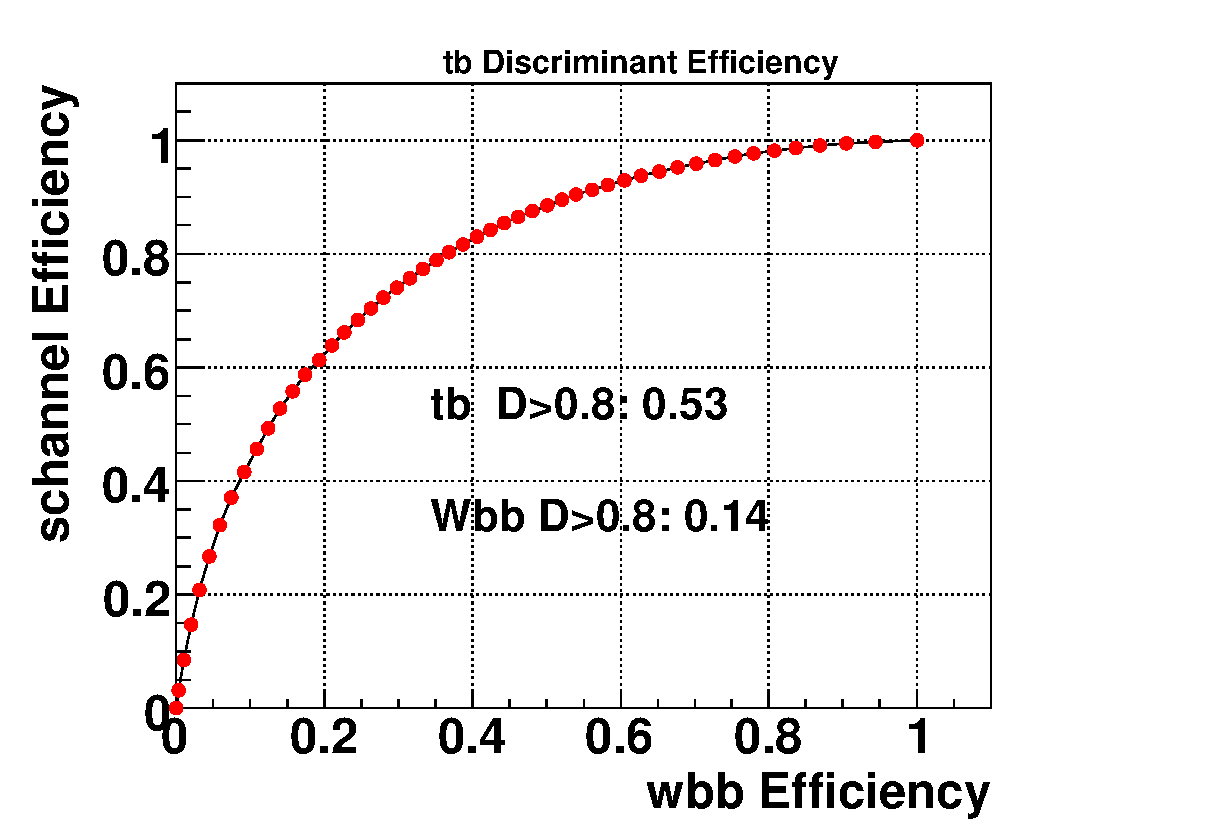
\includegraphics[width=0.49\textwidth]
{eps/MatrixElement/performance/tb_Efficiency__schannel_wbb}
\includegraphics[width=0.49\textwidth]
{eps/MatrixElement/performance/tq_Discriminant__tchannel_wbb}
\includegraphics[width=0.49\textwidth]
{eps/MatrixElement/performance/tq_Efficiency__tchannel_wbb}
\caption{Discriminant plots and efficiency curves for:
first row, $s$-channel vs. $Wbb$ and second row, $t$-channel
vs. $Wbb$. The numbers in the
efficiency curves (right column) represent the fraction of signal or
background the remains after a discriminant cut of 0.8.}
\label{disc_wbb}
\end{figure}

\begin{figure}[!h!tbp]
\includegraphics[width=0.49\textwidth]
{eps/MatrixElement/performance/tb_Discriminant__schannel_wcc}
\includegraphics[width=0.49\textwidth]
{eps/MatrixElement/performance/tb_Efficiency__schannel_wcc}
\includegraphics[width=0.49\textwidth]
{eps/MatrixElement/performance/tq_Discriminant__tchannel_wcc}
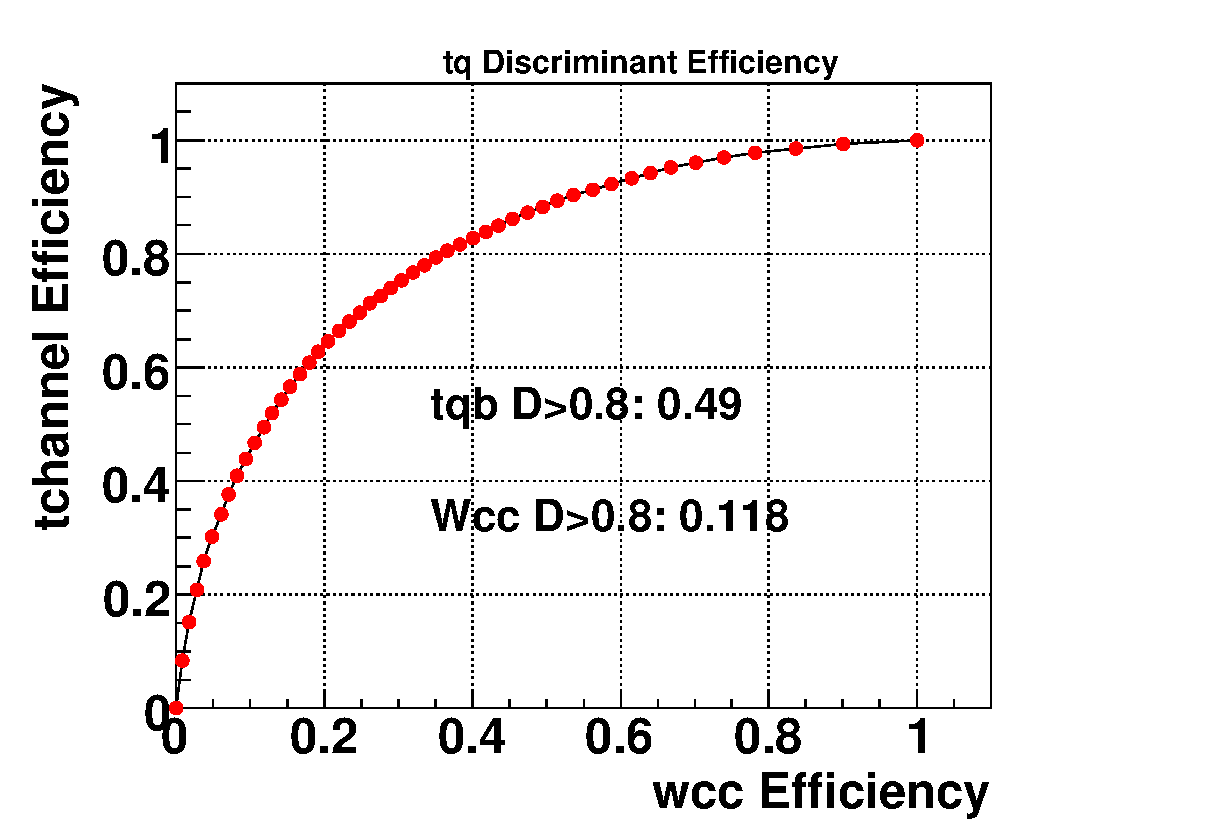
\includegraphics[width=0.49\textwidth]
{eps/MatrixElement/performance/tq_Efficiency__tchannel_wcc}
\caption{Discriminant plots and efficiency curves for:
first row, $s$-channel vs. $Wcc$ and second row, $t$-channel
vs. $Wcc$. The numbers in the
efficiency curves (right column) represent the fraction of signal or
background the remains after a discriminant cut of 0.8.}
\label{disc_wcc}
\end{figure}

\begin{figure}[!h!tbp]
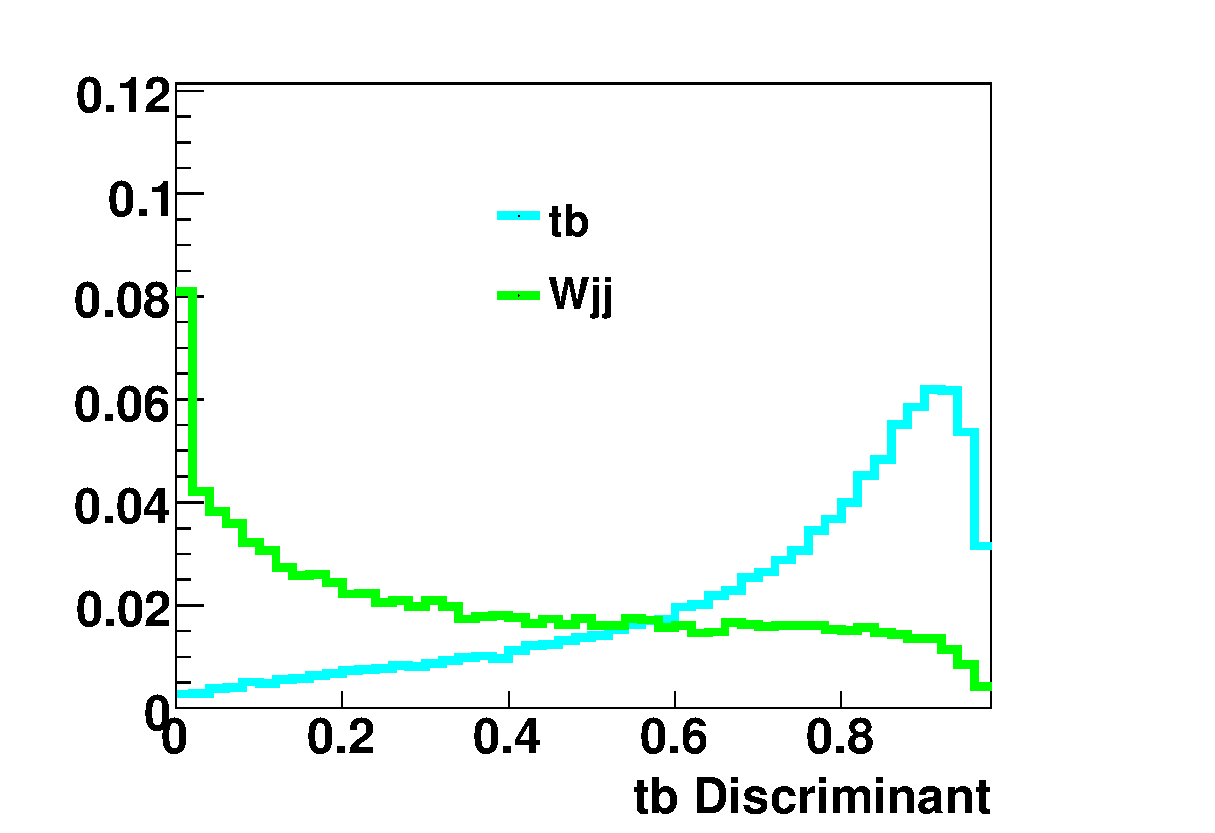
\includegraphics[width=0.49\textwidth]
{eps/MatrixElement/performance/tb_Discriminant__schannel_wjj}
\includegraphics[width=0.49\textwidth]
{eps/MatrixElement/performance/tb_Efficiency__schannel_wjj}
\includegraphics[width=0.49\textwidth]
{eps/MatrixElement/performance/tq_Discriminant__tchannel_wjj}
\includegraphics[width=0.49\textwidth]
{eps/MatrixElement/performance/tq_Efficiency__tchannel_wjj}
\caption{Discriminant plots and efficiency curves for:
first row, $s$-channel vs. $Wjj$ and second row, $t$-channel
vs. $Wjj$. The numbers in the
efficiency curves (right column) represent the fraction of signal or
background the remains after a discriminant cut of 0.8.}
\label{disc_wjj}
\end{figure}

\begin{figure}[!h!tbp]
\includegraphics[width=0.49\textwidth]
{eps/MatrixElement/performance/tb_Discriminant__schannel_qcd}
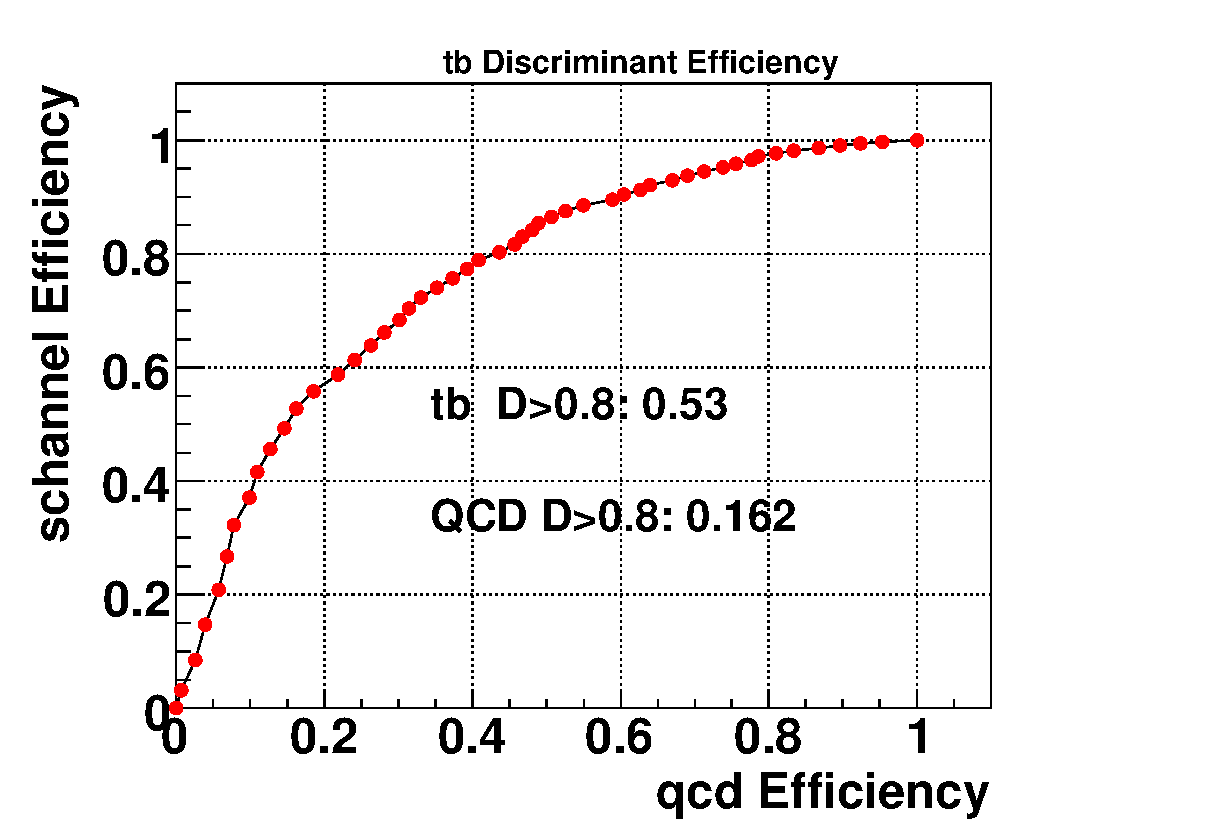
\includegraphics[width=0.49\textwidth]
{eps/MatrixElement/performance/tb_Efficiency__schannel_qcd}
\includegraphics[width=0.49\textwidth]
{eps/MatrixElement/performance/tq_Discriminant__tchannel_qcd}
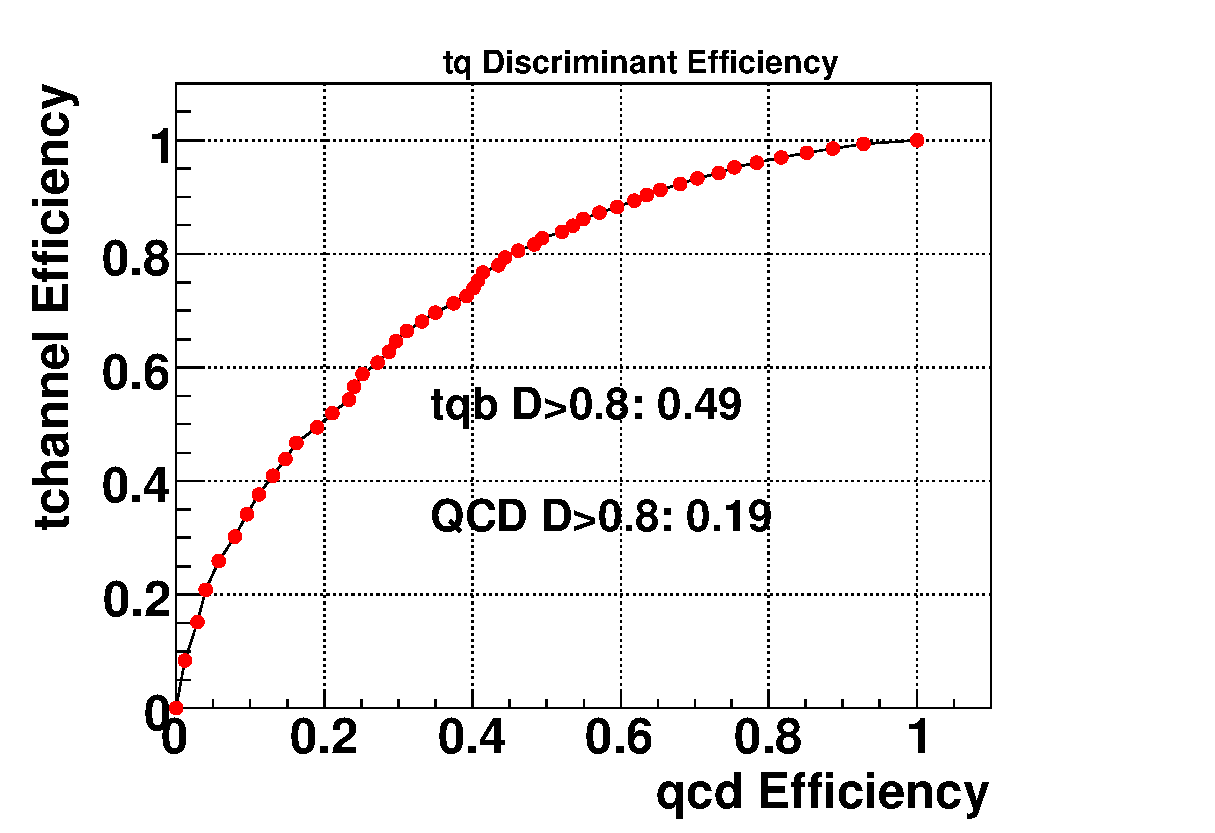
\includegraphics[width=0.49\textwidth]
{eps/MatrixElement/performance/tq_Efficiency__tchannel_qcd}
\caption{Discriminant plots and efficiency curves for:
first row, $s$-channel vs. Multijets and second row, $t$-channel
vs. Multijets. The numbers in the
efficiency curves (right column) represent the fraction of signal or
background the remains after a discriminant cut of 0.8.}
\label{disc_qcd}
\end{figure}

\begin{figure}[!h!tbp]
\includegraphics[width=0.49\textwidth]
{eps/MatrixElement/performance/tb_Discriminant__schannel_dilepton}
\includegraphics[width=0.49\textwidth]
{eps/MatrixElement/performance/tb_Efficiency__schannel_dilepton}
\includegraphics[width=0.49\textwidth]
{eps/MatrixElement/performance/tq_Discriminant__tchannel_dilepton}
\includegraphics[width=0.49\textwidth]
{eps/MatrixElement/performance/tq_Efficiency__tchannel_dilepton}
\caption{Discriminant plots and efficiency curves for:
first row, $s$-channel vs. $\dilepton$ and second row, $t$-channel
vs. $\dilepton$. The numbers in the
efficiency curves (right column) represent the fraction of signal or
background the remains after a discriminant cut of 0.8.}
\label{disc_dilepton}
\end{figure}

\begin{figure}[!h!tbp]
\includegraphics[width=0.49\textwidth]
{eps/MatrixElement/performance/tb_Discriminant__schannel_lepjets}
\includegraphics[width=0.49\textwidth]
{eps/MatrixElement/performance/tb_Efficiency__schannel_lepjets}
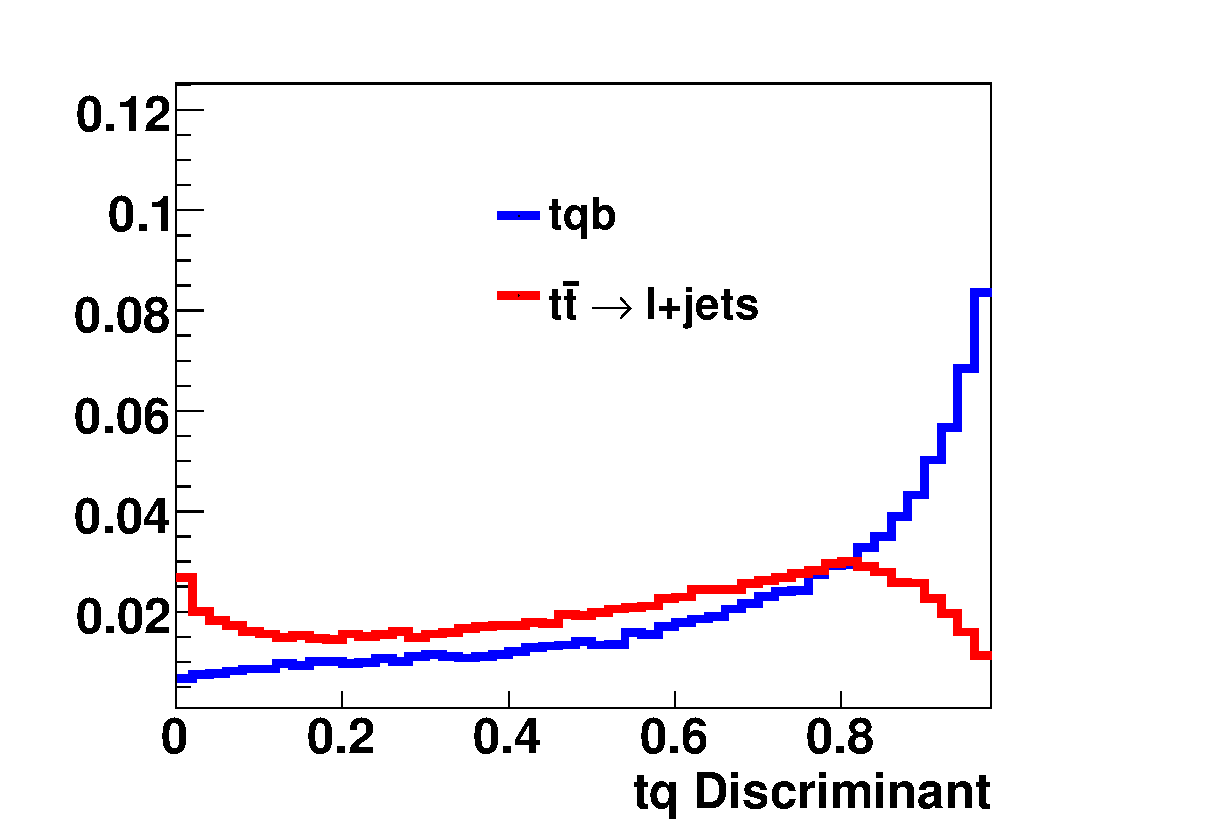
\includegraphics[width=0.49\textwidth]
{eps/MatrixElement/performance/tq_Discriminant__tchannel_lepjets}
\includegraphics[width=0.49\textwidth]
{eps/MatrixElement/performance/tq_Efficiency__tchannel_lepjets}
\caption{Discriminant plots and efficiency curves for:
first row, $s$-channel vs. $\lepjets$ and second row, $t$-channel
vs. $\lepjets$. The numbers in the
efficiency curves (right column) represent the fraction of signal or
background the remains after a discriminant cut of 0.8.}
\label{disc_lepjets}
\end{figure}


\clearpage
\subsection{Two-Dimensional Discriminants}

This analysis uses a two-dimensional (2D) discriminant as the final output where one axis is the $s$-channel discriminant and the other axis is the $t$-channel discriminant value for the event. The 2D discriminant is more powerful than either 1D
projection because it selects events with both $s$ and $t$-channel
characteristics, which helps to further reduce the $W$+jets and
$\ttbar$ background which may have either characteristic but not
necessarily both. Fig.~\ref{tbtqb} shows the 2D discriminant for $s$-channel and $t$-channel Monte Carlo evemts. Figures~\ref{wbbwccwjj} and \ref{qcdtt} show the 2D discriminants for all the backgrounds. The plots are normalized to unit volume.

\begin{figure}[!h!tbp]
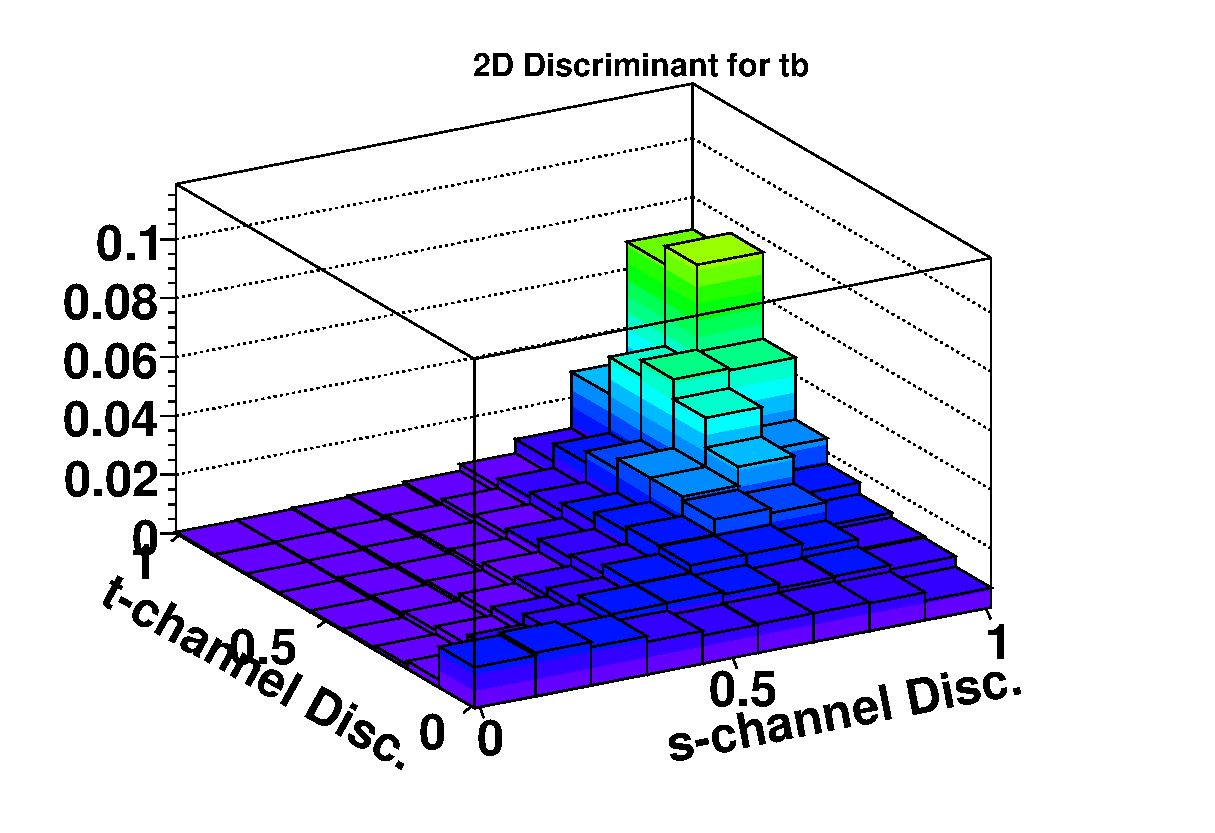
\includegraphics[width=0.49\textwidth]
{eps/MatrixElement/performance/2D-Discriminant_schannel}
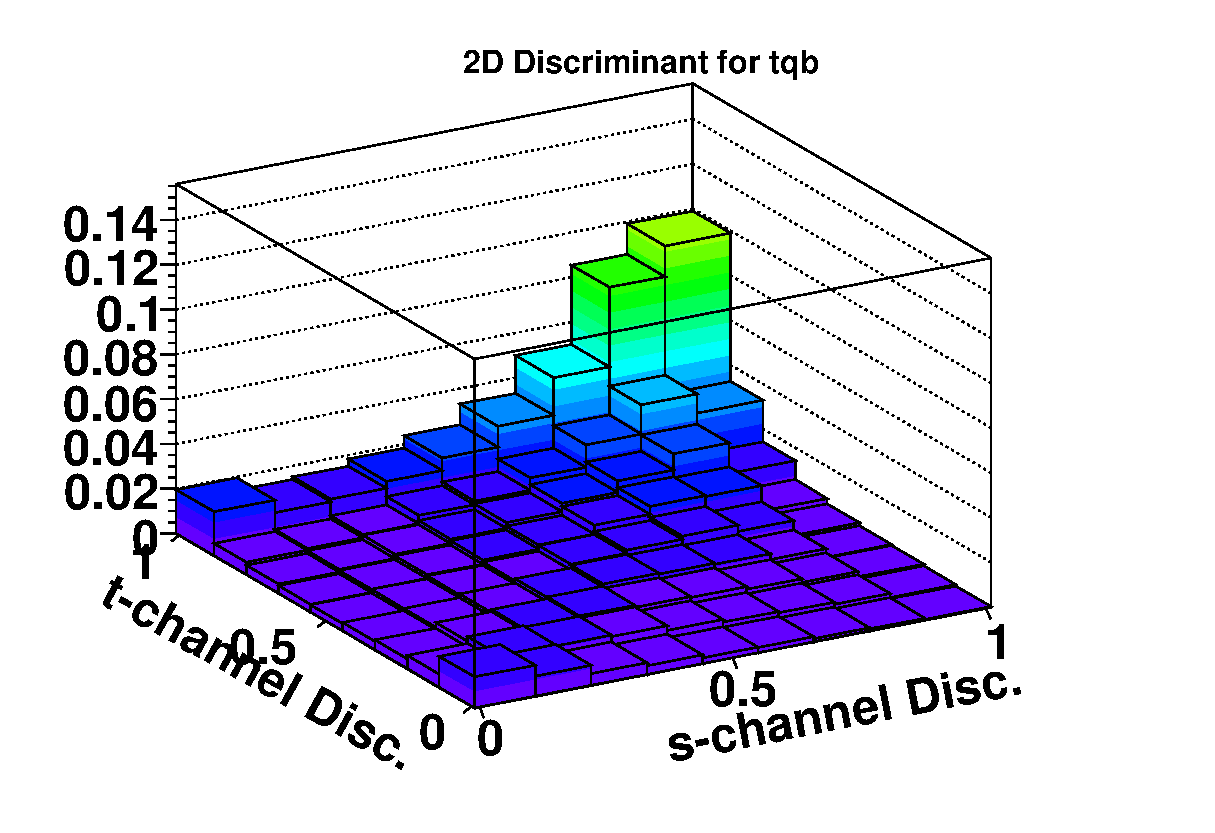
\includegraphics[width=0.49\textwidth]
{eps/MatrixElement/performance/2D-Discriminant_tchannel}
\vspace{-0.1in}
\caption{2D-discriminant templates for: left, $s$-channel , and
right, $t$-channel Monte Carlo events.}
\label{tbtqb}
\end{figure}

\begin{figure}[!h!tbp]
\includegraphics[width=0.49\textwidth]
{eps/MatrixElement/performance/2D-Discriminant_wbb}
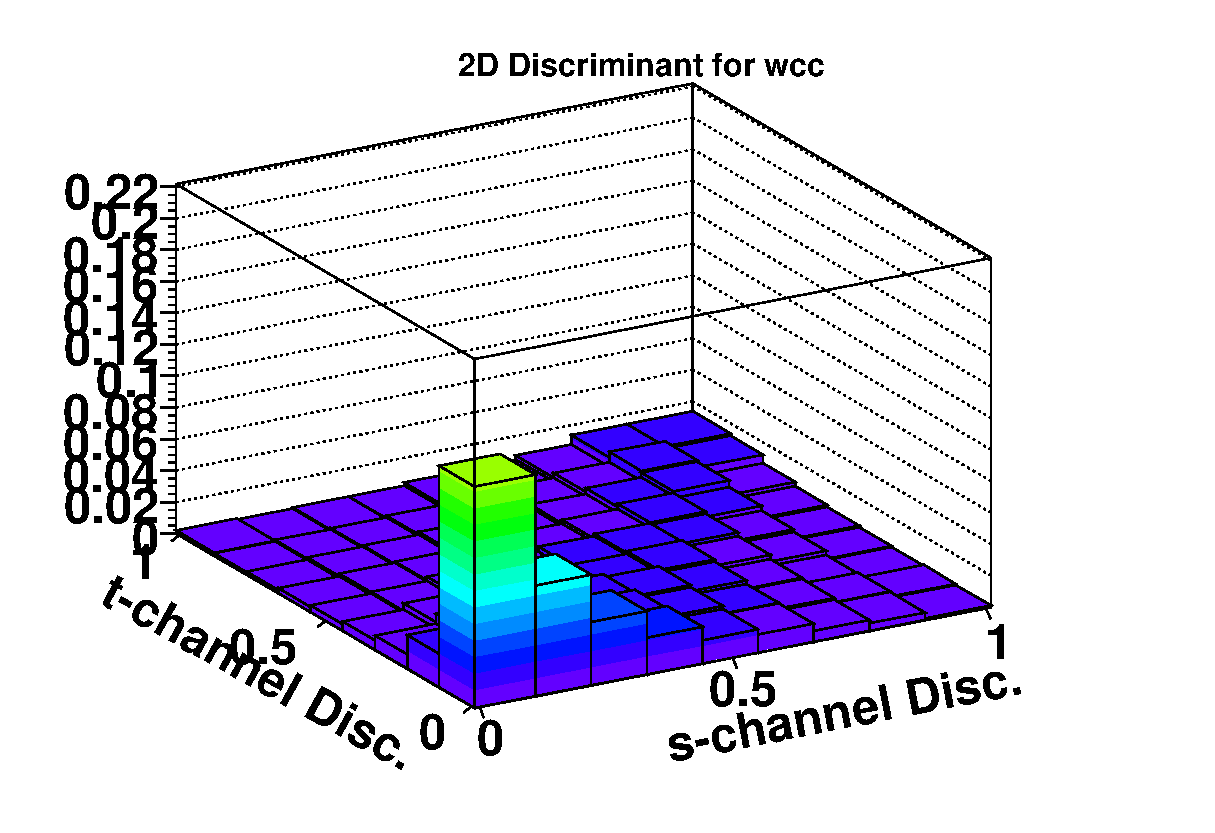
\includegraphics[width=0.49\textwidth]
{eps/MatrixElement/performance/2D-Discriminant_wcc}
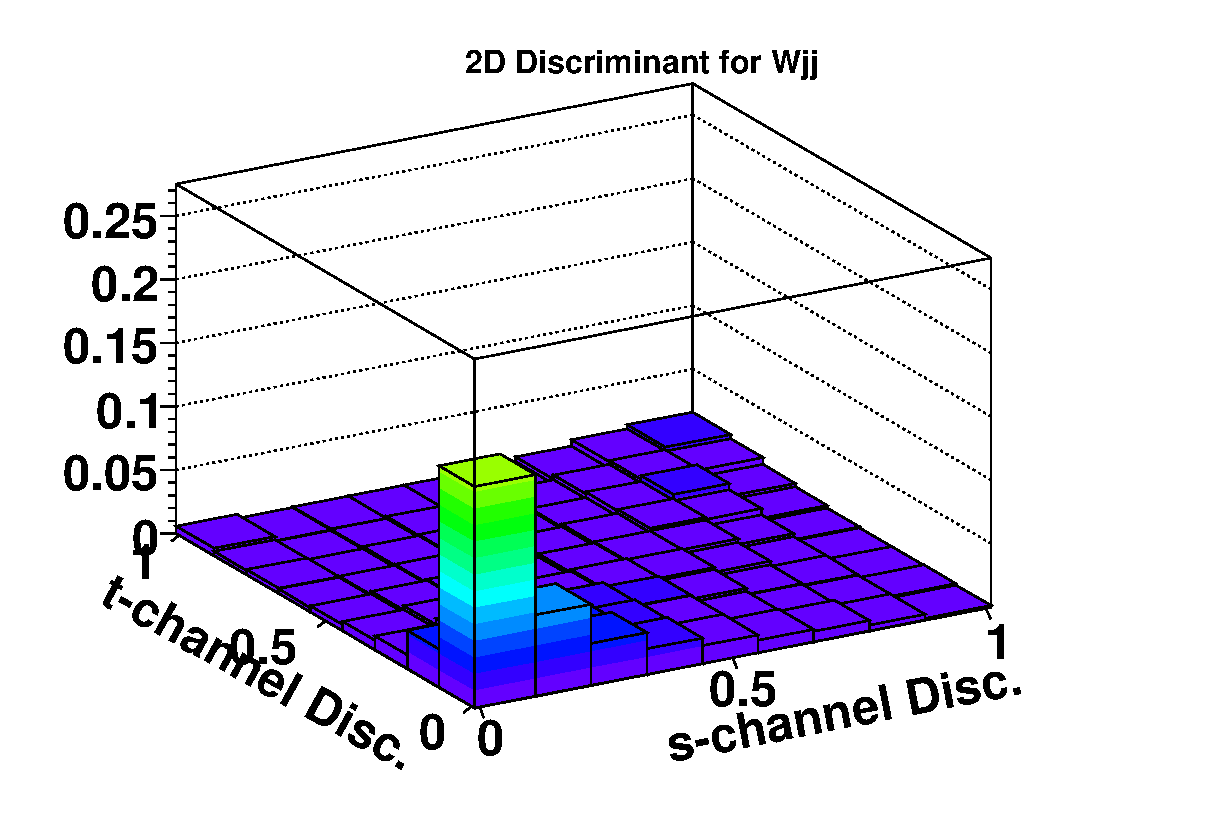
\includegraphics[width=0.49\textwidth]
{eps/MatrixElement/performance/2D-Discriminant_wjj}
\vspace{-0.1in}
\caption{2D-discriminant templates for: top-left,
$Wbb$, top-right, $Wcc$, and bottom-left, $Wjj$ Monte Carlo events.}
\label{wbbwccwjj}
\end{figure}

\begin{figure}[!h!tbp]
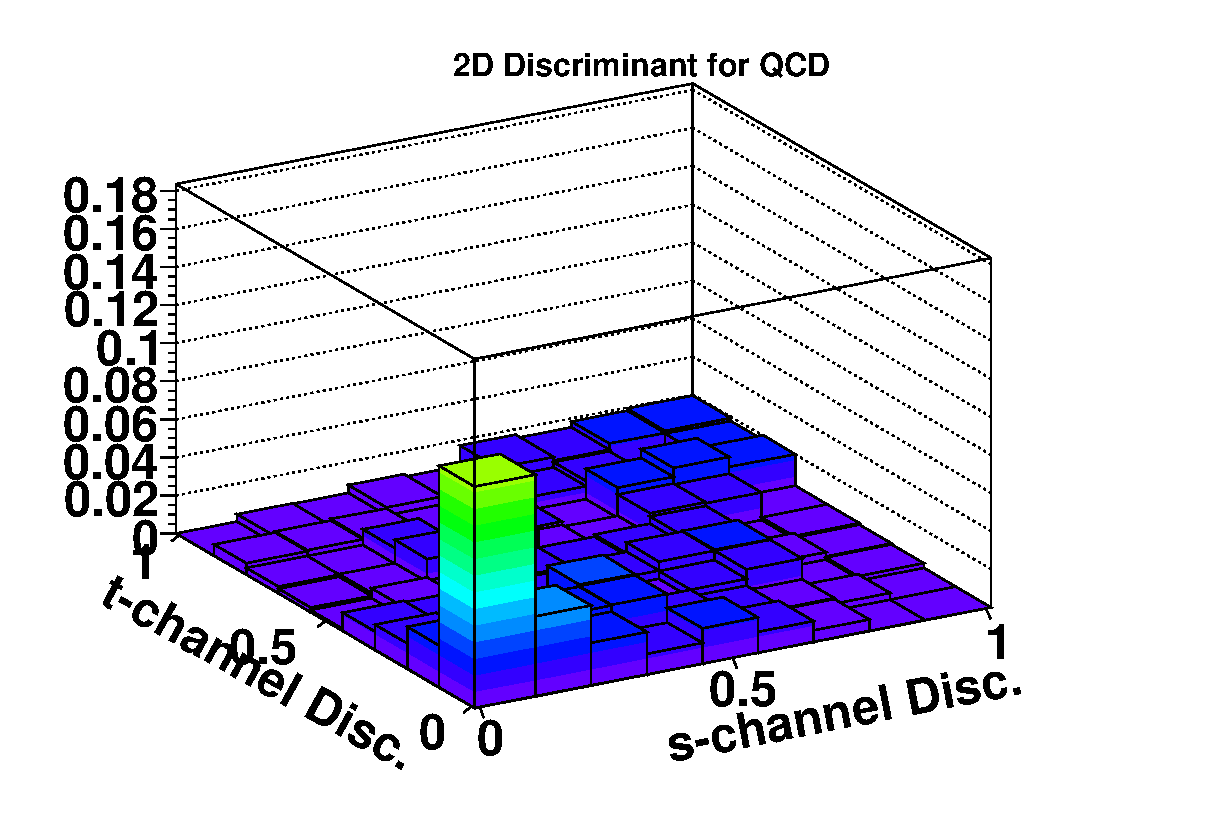
\includegraphics[width=0.49\textwidth]
{eps/MatrixElement/performance/2D-Discriminant_qcd}
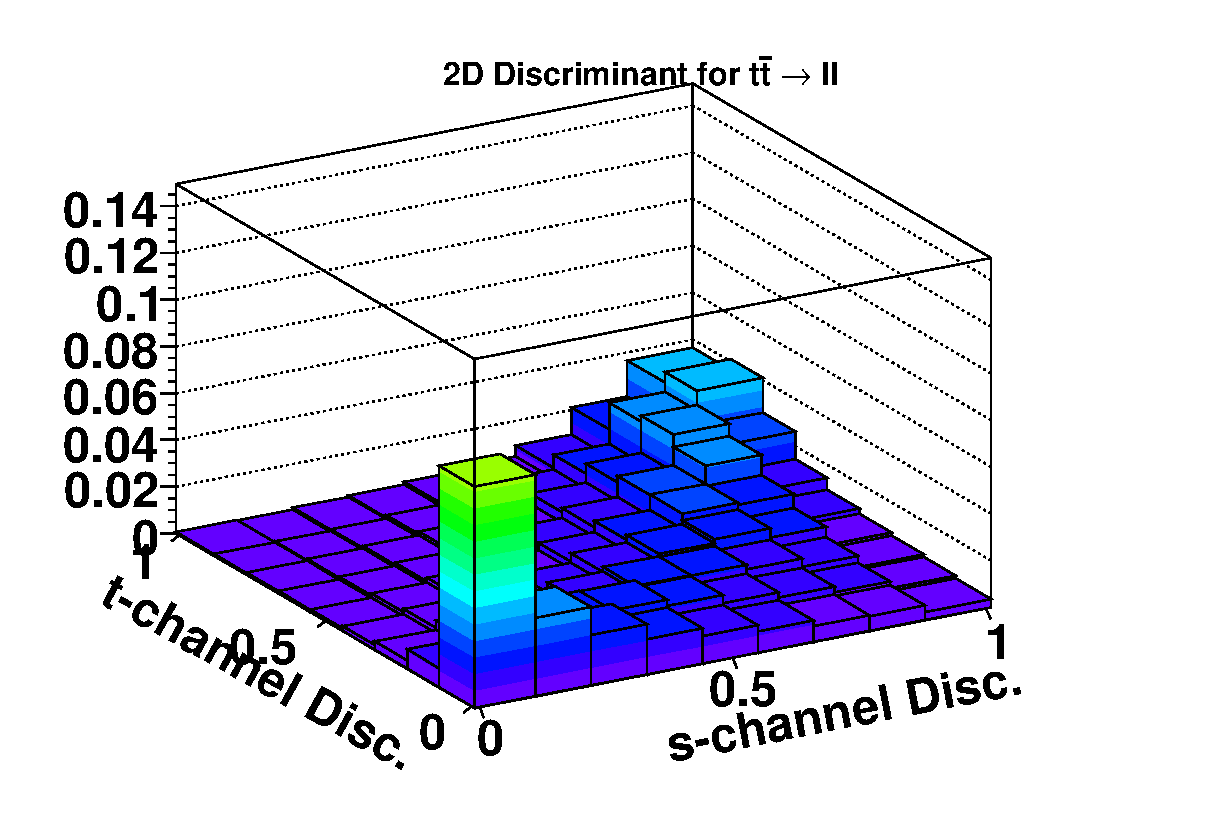
\includegraphics[width=0.49\textwidth]
{eps/MatrixElement/performance/2D-Discriminant_dilepton}
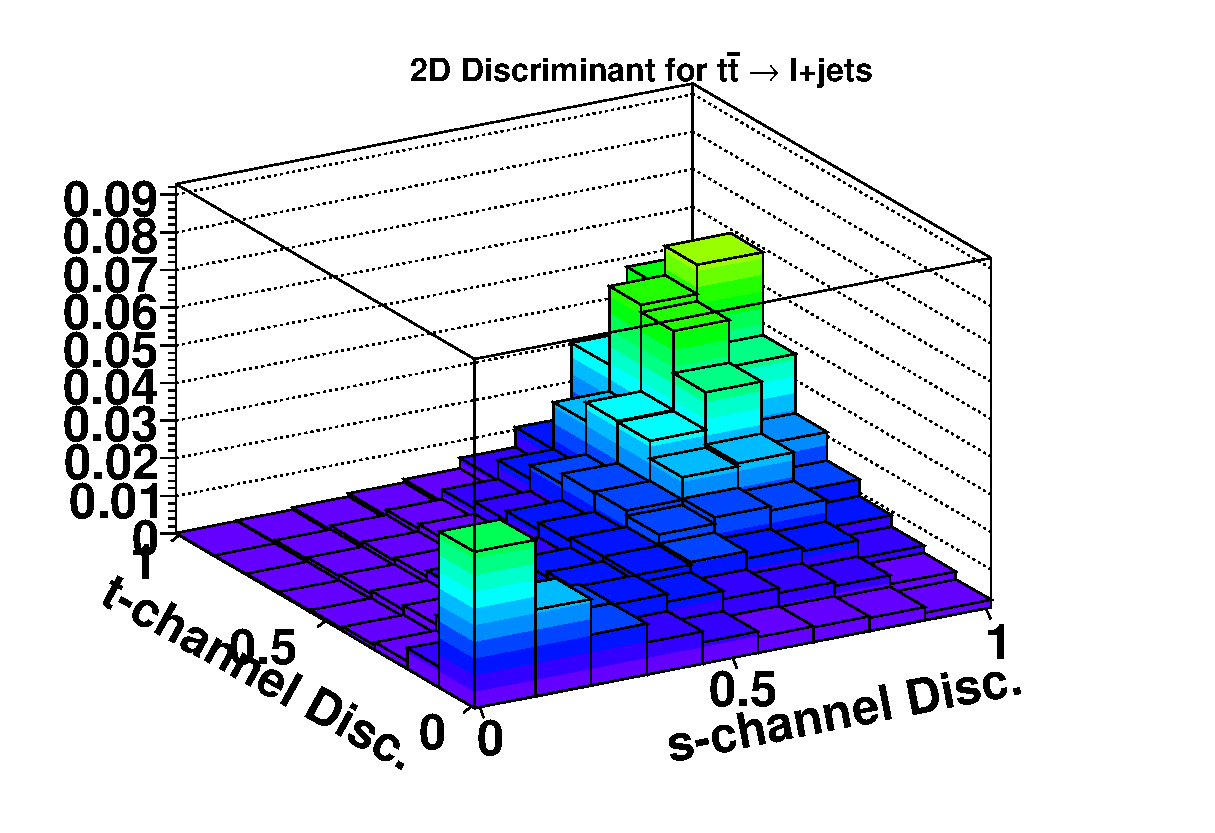
\includegraphics[width=0.49\textwidth]
{eps/MatrixElement/performance/2D-Discriminant_lepjets}
\vspace{-0.1in}
\caption{2D-discriminant templates for: top-left,
multijets events, top-right, $\dilepton$, and bottom-right, $\lepjets$ Monte
Carlo events.}
\label{qcdtt}
\end{figure}


\clearpage
\section{Cross-Check Samples}
\label{crosscheck}

Before a measurement of the single top quark cross section is made, the output of the matrix element analysis is compared between data and background in a region where the signal content is negligible. If the agreement between data and background is good in this sample, there is more confidence that the background is well-modeled in the signal region. In this analysis two background-dominated control
samples are defined, and a comparison between the 1D discriminants in
data and the background model is performed.

These two control samples are selected by applying the nominal event
selection, and requiring an additional cut on the total transverse energy $H_{T}$ defined as

\begin{equation}
H_{T} = p^{\rm{lepton}}_{T} + \rm{M}E_{T} + \sum_{\rm{jets}} p^{jet}_{T}
\end{equation}

The first sample selects events with $H_T<175$~GeV and the second sample selects events with $H_T>300$~GeV,
respectively. The control samples defined with $H_{T}<175$~GeV is referred to as the ``soft $W$+jets'' sample and the sample with $H_{T}>300$~GeV is referred to as the ``hard $W$+jets'' sample. In the case of three-jet events, the ``hard $W$+jets'' sample also contains a
significant fraction of $\ttbar$.

The ``soft $W$+jets'' sample selects low momentum $W$+jets and
multijets events and almost no top-quark events.
Figures~\ref{wjets-cross-2jet} and \ref{wjets-cross-3jet} compare the
$s$-channel and $t$-channel discriminants between data and the background model for
events with two and three jets respectively.

The ``hard $W$+jets'' sample selects mainly $\ttbar$ and high momentum
$W$+jets events. Figures~\ref{ttbar-cross-2jet} and
\ref{ttbar-cross-3jet} compare the $s$-channel and $t$-channel discriminants between
data and the background model for events with two and three jets.

\clearpage
\begin{figure}[!h!tbp]
\includegraphics[width=0.49\textwidth]
{eps/MatrixElement/cross_check/combined/2jet/Wjets_tb_Discriminant}
\includegraphics[width=0.49\textwidth]
{eps/MatrixElement/cross_check/combined/2jet/Wjets_tb_Discriminant_Zoom}
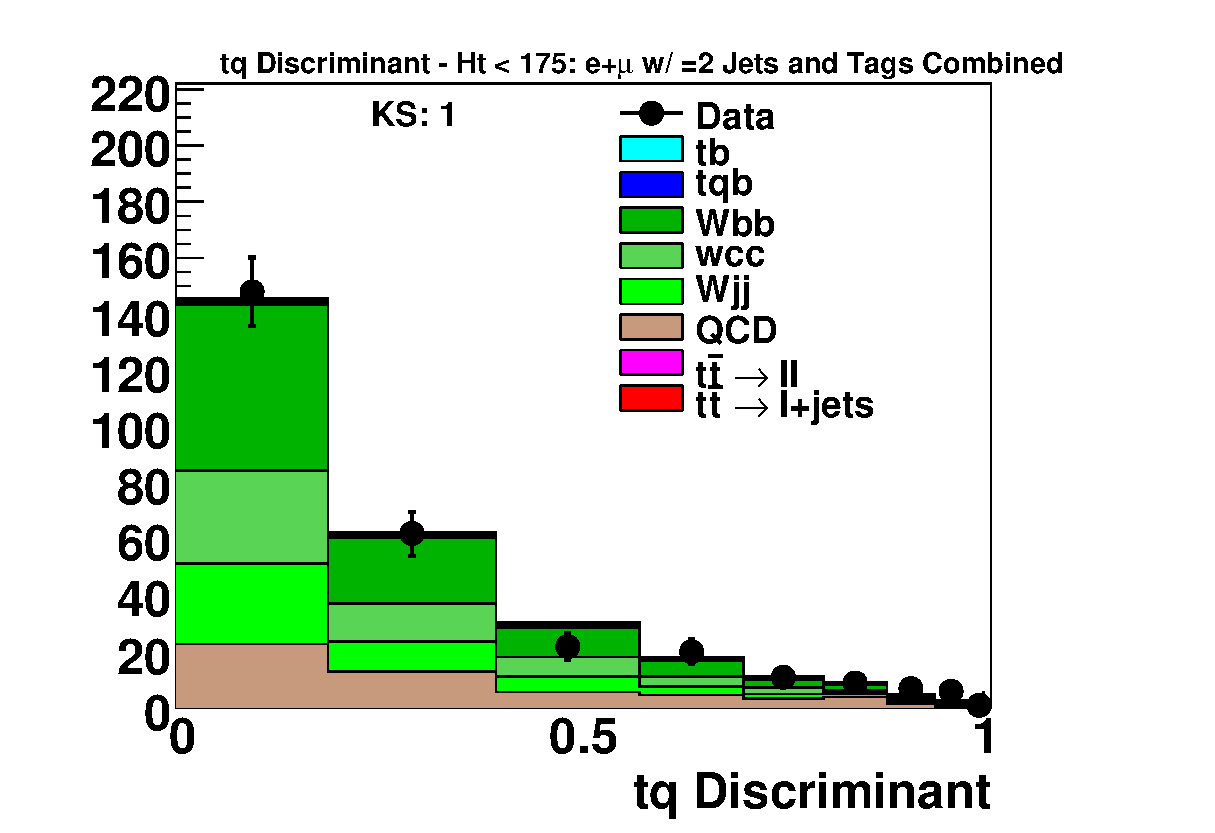
\includegraphics[width=0.49\textwidth]
{eps/MatrixElement/cross_check/combined/2jet/Wjets_tq_Discriminant}
\includegraphics[width=0.49\textwidth]
{eps/MatrixElement/cross_check/combined/2jet/Wjets_tq_Discriminant_Zoom}
\vspace{-0.1in}
\caption{``Soft $W$+jets'' cross-check plots in two-jet
events for the $s$-channel discriminant (upper row) and the $t$-channel discriminant
(lower row). The left column shows the full discriminant region while
the right column shows the high discriminant region above 0.7.}
\label{wjets-cross-2jet}
\end{figure}

\clearpage
\begin{figure}[!h!tbp]
\includegraphics[width=0.49\textwidth]
{eps/MatrixElement/cross_check/combined/3jet/Wjets_tb_Discriminant}
\includegraphics[width=0.49\textwidth]
{eps/MatrixElement/cross_check/combined/3jet/Wjets_tb_Discriminant_Zoom}
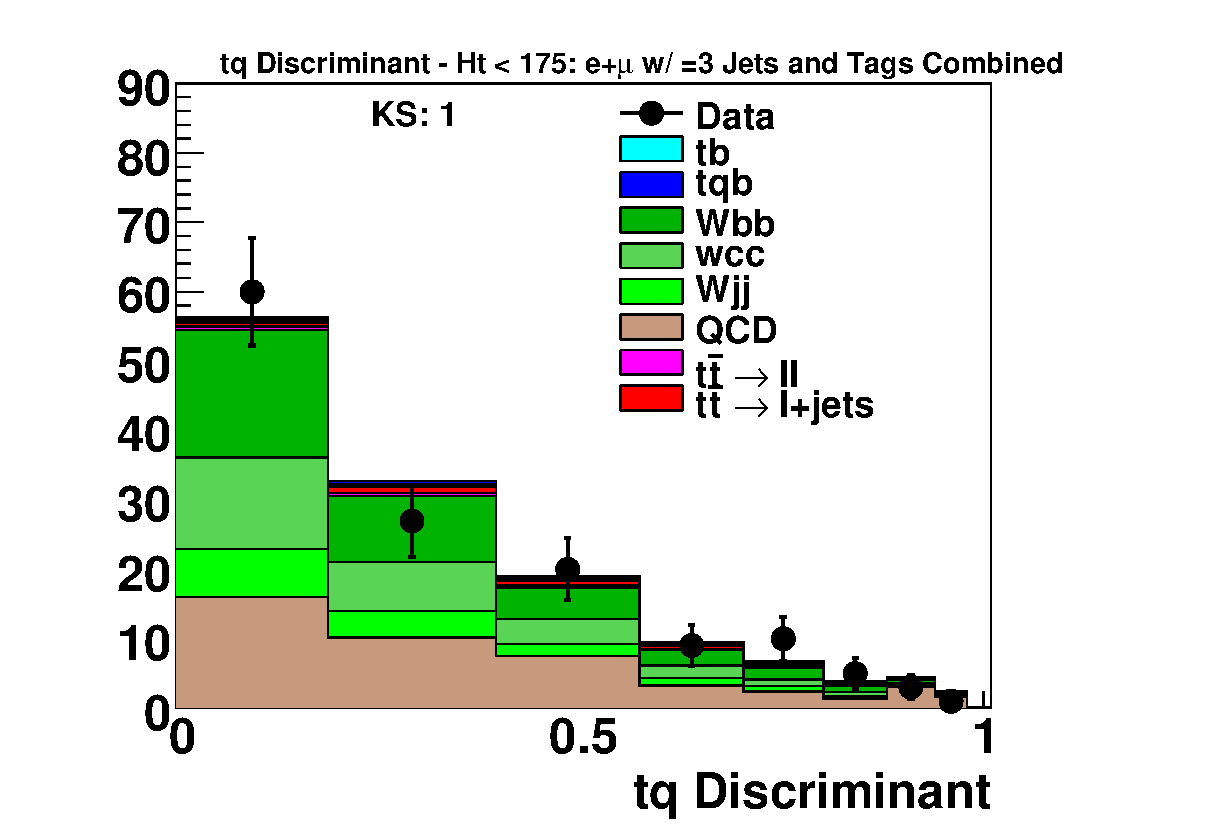
\includegraphics[width=0.49\textwidth]
{eps/MatrixElement/cross_check/combined/3jet/Wjets_tq_Discriminant}
\includegraphics[width=0.49\textwidth]
{eps/MatrixElement/cross_check/combined/3jet/Wjets_tq_Discriminant_Zoom}
\vspace{-0.1in}
\caption{``Soft $W$+jets'' cross-check plots in three-jet
events for the $s$-channel discriminant (upper row) and the $t$-channel discriminant
(lower row). The left column shows the full discriminant region while
the right column shows the high discriminant region above 0.7.}
\label{wjets-cross-3jet}
\end{figure}

\clearpage
\begin{figure}[!h!tbp]
\includegraphics[width=0.49\textwidth]
{eps/MatrixElement/cross_check/combined/2jet/TTbar_tb_Discriminant}
\includegraphics[width=0.49\textwidth]
{eps/MatrixElement/cross_check/combined/2jet/TTbar_tb_Discriminant_Zoom}
\includegraphics[width=0.49\textwidth]
{eps/MatrixElement/cross_check/combined/2jet/TTbar_tq_Discriminant}
\includegraphics[width=0.49\textwidth]
{eps/MatrixElement/cross_check/combined/2jet/TTbar_tq_Discriminant_Zoom}
\vspace{-0.1in}
\caption{``Hard $W$+jets'' cross-check plots in two-jet
events for the $s$-channel discriminant (upper row) and the $t$-channel discriminant
(lower row). The left column shows the full discriminant region while
the right column shows the high discriminant region above 0.7.}
\label{ttbar-cross-2jet}
\end{figure}

\clearpage
\begin{figure}[!h!tbp]
\includegraphics[width=0.49\textwidth]
{eps/MatrixElement/cross_check/combined/3jet/TTbar_tb_Discriminant}
\includegraphics[width=0.49\textwidth]
{eps/MatrixElement/cross_check/combined/3jet/TTbar_tb_Discriminant_Zoom}
\includegraphics[width=0.49\textwidth]
{eps/MatrixElement/cross_check/combined/3jet/TTbar_tq_Discriminant}
\includegraphics[width=0.49\textwidth]
{eps/MatrixElement/cross_check/combined/3jet/TTbar_tq_Discriminant_Zoom}
\vspace{-0.1in}
\caption{``Hard $W$+jets'' cross-check plots in three-jet
events for the $s$-channel discriminant (upper row) and the $t$-channel discriminant
(lower row). The left column shows the full discriminant region while
the right column shows the high discriminant region above 0.7.}
\label{ttbar-cross-3jet}
\end{figure}

\clearpage
\section{Matrix Element Discriminants}
\label{matrixelementresults}

This section presents the matrix element discriminants for all events in each analysis channel. Figures~\ref{e21_2j} and~\ref{e21_3j} show the $s$-channel and $t$-channel
discriminants for the combined $e$,$\mu$ w/ $\geq1$ $B$-tag events for two-jet
and three-jet events where the data distributions may be compared to
the background model.  The SM prediction for single top quark
production has been added to the background sum in the plots. The
individual channel plots for the 1D discriminants are shown in
Appendix~\ref{Channel}.

\vspace{-0.05in}
\begin{figure}[!h!tbp]
\includegraphics[width=0.49\textwidth]
{eps/MatrixElement/output/2jet/All_tb_Discriminant.eps}
\includegraphics[width=0.49\textwidth]
{eps/MatrixElement/output/2jet/All_tb_Discriminant_Zoom.eps}
\includegraphics[width=0.49\textwidth]
{eps/MatrixElement/output/2jet/All_tq_Discriminant.eps}
\includegraphics[width=0.49\textwidth]
{eps/MatrixElement/output/2jet/All_tq_Discriminant_Zoom.eps}
\vspace{-0.1in}
\caption{Discriminant plots for the e+$\mu$ channel with two jets and
$\geq$~1 $B$~tag. Upper row: $s$-channel discriminant; lower row: $tq$
discriminant. Left column: full output range; right column: close-up
of the high end of the distributions.}
\label{e21_2j}
\end{figure}

\vspace{-0.05in}
\begin{figure}[!h!tbp]
\includegraphics[width=0.49\textwidth]
{eps/MatrixElement/output/3jet/All_tb_Discriminant.eps}
\includegraphics[width=0.49\textwidth]
{eps/MatrixElement/output/3jet/All_tb_Discriminant_Zoom.eps}
\includegraphics[width=0.49\textwidth]
{eps/MatrixElement/output/3jet/All_tq_Discriminant.eps}
\includegraphics[width=0.49\textwidth]
{eps/MatrixElement/output/3jet/All_tq_Discriminant_Zoom.eps}
\vspace{-0.1in}
\caption{Discriminant plots for the e+$\mu$ channel with three jets
and $\geq$~1 $b$~tag. Upper row: $s$-channel discriminant; lower row: $tq$
discriminant. Left column: full output range; right column: close-up
of the high end of the distributions.}
\label{e21_3j}
\end{figure}

\clearpage
After the matrix element discriminant has been calculated it is
possible to select events in data and
Monte Carlo to see if they are consistent with single top quark
production. For this section, an event is considered very single top
quark like if both the $s$-channel and $t$-channel discriminants are
greater than 0.7. Similarly, an event is considered background like if
both discriminants are less than 0.4. Figure~\ref{top-mass} shows the
invariant mass of the lepton, neutrino, and tagged jet before and
after the discriminant cut, and Fig.~\ref{q-eta} shows the
lepton-charge times pseudorapidity of the untagged jet. In both cases the background dominated samples show no evidence for top quarks in the event while the signal enhanced samples are re-shaped to look like the expected single top distributions.

\begin{figure}[!h!tbp]
\includegraphics[width=0.49\textwidth]
{eps/MatrixElement/topovars/BTaggedTopMass_0.eps}
\includegraphics[width=0.49\textwidth]
{eps/MatrixElement/topovars/BTaggedTopMass_-0.4.eps}
\includegraphics[width=0.49\textwidth]
{eps/MatrixElement/topovars/BTaggedTopMass_0.7.eps}
\vspace{-0.1in}
\caption{Invariant mass of the lepton, neutrino, and tagged
jet for all events (upper left plot), for events with $D < 0.4$ (upper right plot), and events with $D > 0.7$ (bottom left plot).}
\label{top-mass}
\end{figure}

%\vspace{0.1in}
\begin{figure}[!h!tbp]
\includegraphics[width=0.49\textwidth]
{eps/MatrixElement/topovars/QTimesEta_0.eps}
\includegraphics[width=0.49\textwidth]
{eps/MatrixElement/topovars/QTimesEta_-0.4.eps}
\includegraphics[width=0.49\textwidth]
{eps/MatrixElement/topovars/QTimesEta_0.7.eps}
\vspace{-0.1in}
\caption{Lepton charge multiplied by the pseudorapidity of the untagged
jet for all events (upper left plot), for events with $D < 0.4$ (upper right
plot), and events with $D > 0.7$ (bottom left plot). The number of observed
events is different from the $b$-tagged top mass plot because this
variable is only defined for events with at least one untagged jet.}
\label{q-eta}
\end{figure}

